\documentclass[a4paper,10pt,landscape]{article}
\usepackage[table,xcdraw]{xcolor}
\usepackage{palatino}
\usepackage{multicol}
\usepackage{multirow}
\usepackage{calc}
\usepackage{ifthen}
\usepackage[landscape]{geometry}
\usepackage{graphicx}
\usepackage{amsmath, amssymb, amsthm}
\usepackage{latexsym, marvosym}
\usepackage{pifont}
\usepackage{lscape}
\usepackage{dsfont}
\usepackage{graphicx}
\usepackage{array}
\newcolumntype{L}[1]{>{\raggedright\let\newline\\\arraybackslash\hspace{0pt}}m{#1}}
\newcolumntype{C}[1]{>{\centering\let\newline\\\arraybackslash\hspace{0pt}}m{#1}}
\newcolumntype{R}[1]{>{\raggedleft\let\newline\\\arraybackslash\hspace{0pt}}m{#1}}
\usepackage{booktabs}
\usepackage[bottom]{footmisc}
\usepackage{tikz}
\usetikzlibrary{shapes}
\usepackage{pdfpages}
\usepackage{wrapfig}
\usepackage{enumitem}
\setlist[description]{leftmargin=0pt}
\usepackage{xfrac}
\usepackage[pdftex,
            pdfauthor={Janus Advincula}
            ]{hyperref}
\usepackage[
            open,
            openlevel=2
            ]{bookmark}
\usepackage{relsize}
\usepackage{longtable}
\usepackage{rotating}

 \newcommand\independent{\protect\mathpalette{\protect\independenT}{\perp}}
    \def\independenT#1#2{\mathrel{\setbox0\hbox{$#1#2$}%
    \copy0\kern-\wd0\mkern4mu\box0}} 
            
\newcommand{\noin}{\noindent}    
\newcommand{\logit}{\textrm{logit}} 
\newcommand{\var}{\textrm{Var}}
\newcommand{\cov}{\textrm{Cov}} 
\newcommand{\corr}{\textrm{Corr}} 
\newcommand{\N}{\mathcal{N}}
\newcommand{\Bern}{\textrm{Bern}}
\newcommand{\Bin}{\textrm{Bin}}
\newcommand{\Beta}{\textrm{Beta}}
\newcommand{\Gam}{\textrm{Gamma}}
\newcommand{\Expo}{\textrm{Expo}}
\newcommand{\Pois}{\textrm{Pois}}
\newcommand{\Unif}{\textrm{Unif}}
\newcommand{\Geom}{\textrm{Geom}}
\newcommand{\NBin}{\textrm{NBin}}
\newcommand{\Hypergeometric}{\textrm{HGeom}}
\newcommand{\HGeom}{\textrm{HGeom}}
\newcommand{\Mult}{\textrm{Mult}}

\geometry{top=.4in,left=.2in,right=.2in,bottom=.4in}

\pagestyle{empty}
\makeatletter
\renewcommand{\section}{\@startsection{section}{1}{0mm}%
                                {-1ex plus -.5ex minus -.2ex}%
                                {0.5ex plus .2ex}%x
                                {\normalfont\large\bfseries}}
\renewcommand{\subsection}{\@startsection{subsection}{2}{0mm}%
                                {-1explus -.5ex minus -.2ex}%
                                {0.5ex plus .2ex}%
                                {\normalfont\normalsize\bfseries}}
\renewcommand{\subsubsection}{\@startsection{subsubsection}{3}{0mm}%
                                {-1ex plus -.5ex minus -.2ex}%
                                {1ex plus .2ex}%
                                {\normalfont\small\bfseries}}
\makeatother

\setcounter{secnumdepth}{0}

\setlength{\parindent}{0pt}
\setlength{\parskip}{0pt plus 0.5ex}

% -----------------------------------------------------------------------

\usepackage{titlesec}

\titleformat{\section}
{\color{blue}\normalfont\large\bfseries}
{\color{blue}\thesection}{1em}{}
\titleformat{\subsection}
{\color{violet}\normalfont\normalsize\bfseries}
{\color{violet}\thesection}{1em}{}
% Comment out the above 5 lines for black and white

\begin{document}

\raggedright
\footnotesize
\begin{multicols*}{3}

% multicol parameters
% These lengths are set only within the two main columns
%\setlength{\columnseprule}{0.25pt}
\setlength{\premulticols}{1pt}
\setlength{\postmulticols}{1pt}
\setlength{\multicolsep}{1pt}
\setlength{\columnsep}{2pt}

%%%%%%%%%%%%%%%%%%%%%%%%%%%%%%%%%%%%
%%% TITLE
%%%%%%%%%%%%%%%%%%%%%%%%%%%%%%%%%%%%

\begin{center}
    {\color{blue} \Large{\textbf{14.310x Data Analysis for Social Scientists}}} \\
   % {\Large{\textbf{Probability Cheatsheet}}} \\
    % comment out line with \color{blue} and uncomment above line for b&w
\end{center}

%%%%%%%%%%%%%%%%%%%%%%%%%%%%%%%%%%%%
%%% ATTRIBUTIONS
%%%%%%%%%%%%%%%%%%%%%%%%%%%%%%%%%%%%

\scriptsize

This is a cheat sheet for data analysis based on the online course given by Prof. Esther Duflo and Prof. Sara Ellison. Compiled by Janus B. Advincula.

\begin{center}
    Last Updated \today
\end{center}

% Cheatsheet format from
% http://www.stdout.org/$\sim$winston/latex/

%%%%%%%%%%%%%%%%%%%%%%%%%%%%%%%%%%%%
%%% BEGIN CHEATSHEET
%%%%%%%%%%%%%%%%%%%%%%%%%%%%%%%%%%%%


\section{Module 1}\smallskip \hrule height 1pt \smallskip

\subsection{Introduction}

\begin{itemize}[noitemsep, topsep=0pt]
	\item Data is plentiful.
	\item Data is beautiful.
	\item Data is insightful.
	\item Data is powerful.
	\item Data can be deceitful.
\end{itemize}

\subsubsection{Causation vs. Correlation}
\begin{itemize}[noitemsep, topsep=0pt]
	\item Correlation is not causality.
	\item A causal {\it story} is not causality either.
	\item Even more sophisticated data use may still not be causality.
\end{itemize}

\subsubsection{What We Need to Learn}
\begin{itemize}[noitemsep, topsep=0pt]
	\item How do we model the processes that might have generated our data?
	\begin{itemize}[noitemsep, topsep=0pt]
		\item[-] Probability
	\end{itemize}
	\item How do we summarize and describe data, and try to uncover what process may have generated it?
	\begin{itemize}[noitemsep, topsep=0pt]
		\item[-] Statistics
	\end{itemize}
	\item How do we uncover pattern between variables?
	\begin{itemize}[noitemsep, topsep=0pt]
		\item[-] Exploratory data analysis
		\item[-] Econometrics
	\end{itemize}
\end{itemize}


\section{Module 2} \smallskip \hrule height 1pt \smallskip

\subsection{Fundamentals of Probability}

\begin{description}
	\item A {\bf sample space} $S$ is a collection of all possible outcomes of an experiment.
	\item An {\bf event} $A$ is any collection of outcomes (including individual outcomes, the entire sample space, the null set).
	\item Useful results:
	\begin{itemize}[itemsep=0.25pt,topsep=0.5pt]
		\item If $A\subset B$, then $A\cup B=B$.
		\item If $A\subset B$ and $B\subset A$, then $A=B$.
		\item If $A\subset B$, then $A\cap B=AB=A$.
		\item $A\cup A^c=S$
	\end{itemize}
	\item $A$ and $B$ are {\it mutually exclusive} ({\bf disjoint}) if they have no outcomes in common.
	\item $A$ and $B$ are {\it exhaustive} ({\bf complementary}) if their union is $S$.
\end{description}
\subsubsection*{Probability}
\begin{description}
	\item We will assign to every event $A$ a number $\mathbb{P}\left(A\right)$, which is the probability the event will occur $\left(\mathbb{P}:S\rightarrow R\right)$.
	\item We require that:
	\begin{enumerate}
		\item $\mathbb{P}(A)\geq0$ for all $A\subset S$
		\item $\mathbb{P}(S)=1$
		\item For any sequence of disjoint sets $A_1, A_2,\dots,$ $$\mathbb{P}\left(\bigcap_iA_i\right)=\sum_{i}\mathbb{P}\left(A_i\right)$$
	\end{enumerate}
	\item A {\bf probability} on a sample space $S$ is a collection of numbers $\mathbb{P}(A)$ that satisfy axioms 1-3.
	\item[Counting] ~
	\begin{enumerate}
		\item If an experiment has two parts, first one having $m$ possibilities and, regardless of the outcome in the first part, the second one having $n$ possibilities, then the experiment has $m\times n$ possible outcomes.
		\item Any ordered arrangement of objects is called a {\bf permutation}. The number of different permutations of $N$ objects is $N!$. The number of different permutations of $n$ objects taken from $N$ objects is $\dfrac{N!}{(N-n)!}$.
		\item Any unordered arrangement of objects is called a {\bf combination}. The number of different combinations of $n$ objects taken from $N$ objects is $\dfrac{N!}{(N-n)!n!}$. We typically denote this $\dbinom{N}{n}$.
	\end{enumerate}
	\item[Properties:] ~
	\begin{itemize}[itemsep=0.5pt]
		\item $\mathbb{P}\left(A^c\right)=1-\mathbb{P}\left(A\right)$
		\item $\mathbb{P}\left(\emptyset\right)=0$
		\item If $A\subset B$ then $\mathbb{P}\left(A\right)\leq\mathbb{P}\left(B\right)$
		\item For all $A$, $0\leq\mathbb{P}\left(A\right)\leq1$
		\item $\mathbb{P}\left(A\cup B\right)=\mathbb{P}\left(A\right)+\mathbb{P}\left(B\right)-\mathbb{P}\left(AB\right)$
		\item $\mathbb{P}\left(AB^c\right)=\mathbb{P}\left(A\right)-\mathbb{P}\left(AB\right)$
	\end{itemize}
	\item[Independence] Events $A$ and $B$ are {\it independent} if $\mathbb{P}\left(AB\right)=\mathbb{P}\left(A\right)\mathbb{P}\left(B\right)$.
	\item[Theorem] If $A$ and $B$ are independent, $A$ and $B^c$ are also independent.
	\item[Conditional Probability] The {\it probability of $A$ conditional on $B$} is
	$$\mathbb{P}\left(A|B\right)=\frac{\mathbb{P}\left(AB\right)}{\mathbb{P}\left(B\right)},\quad\mathbb{P}\left(B\right)>0.$$
	\item If $A$ and $B$ are independent and $\mathbb{P}\left(B\right)>0$, then $$\mathbb{P}\left(A|B\right)=\frac{\mathbb{P}\left(AB\right)}{\mathbb{P}\left(B\right)}=\frac{\mathbb{P}\left(A\right)\mathbb{P}\left(B\right)}{\mathbb{P}\left(B\right)}=\mathbb{P}\left(A\right).$$
	\item[Bayes' Theorem] ~
	$$\mathbb{P}\left(A|B\right)=\frac{\mathbb{P}\left(B|A\right)\mathbb{P}\left(A\right)}{\mathbb{P}\left(B|A\right)\mathbb{P}\left(A\right)+\mathbb{P}\left(B|A^c\right)\mathbb{P}\left(A^c\right)}$$
	($A$ and $A^c$ form a partition of $S$.)
\end{description}

\subsection{Random Variables, Distributions, and Joint\newline Distributions}

\begin{description}
	\item A {\bf random variable} is a real-valued function whose domain is the sample space.
	\item A {\bf discrete} random variable can take on only a finite or countable infinite number of values.
	\item A random variable that can take on any value in some interval, bounded or unbounded, of the real line is called a {\bf continuous} random variable.
	\item[Hypergeometric Distribution] $X\sim\mathcal{H}\left(N, K, n\right)$
	$$f_X(x)=\dfrac{\binom{K}{x}\binom{N-K}{n-x}}{\binom{N}{n}},\quad x=\max\left(0,n+K-N\right),\dots,\min\left(n,K\right)$$
	The hypergeometric distribution describes the number of "successes" in $n$ trials where you're sampling without replacement from a sample of size $N$ whose initial probability of success was $K/N$.
	\item[Binomial Distribution] $X\sim\mathcal{B}(n,p)$
	$$f_X(x)=\binom{n}{x}p^x(1-p)^{n-x},\quad x=0,1,\dots,n$$
	The binomial distribution describes the number of "successes in $n$ trials where the trials are independent and the probability of success in each is $p$.
	\item The {\bf probability function} (PF) of $X$, where $X$ is a discrete random variable, is the function $f_X$ such that for any real number $x$, $f_X(x)=\mathbb{P}(X=x)$.
	\item[Properties:] ~
	\begin{itemize}
		\item $0\leq f_X(x_i)\leq1$
		\item $\sum\limits_{i}f_X(x_i)=1$
		\item $\mathbb{P}(A)=\mathbb{P}(X\subset A)=\sum\limits_{A}f_X(x_i)$
		\item $\mathbb{P}(X=x)=0$ for any $x$ if $X$ is continuous.
	\end{itemize}
	\item The {\bf density} or {\bf probability density function} (PDF) is the continuous analog to the discrete PF in many ways.
	\item A random variable $X$ is {\bf continuous} if there exists a non-negative function $f_X$ such that for any interval $A\subset R$, 
	$$\mathbb{P}(X\subset A)=\int_{A}f_X(x)dx.$$
	\item[Properties:] ~
	\begin{itemize}
		\item $0\leq f_X(x)$
		\item $\int f_X(x)dx=1$
		\item $\mathbb{P}(A)=\mathbb{P}(a\leq X\leq b)=\int_{A}f_X(x)dx$
	\end{itemize}
	\item The {\bf cumulative distribution function} (CDF) $F_X$ of a random variable $X$ is defined for each $x$ as $$F_X(x)=\mathbb{P}(X\leq x).$$
	\item[Properties:] ~
	\begin{itemize}
		\item $0\leq F_X(x)\leq 1$
		\item $F_X(x)$ is non-decreasing in $x$
		\item $\lim\limits_{x\rightarrow-\infty}F_X(x)=0$
		\item $\lim\limits_{x\rightarrow\infty}F_X(x)=1$
		\item $F_X(x)$ is right continuous.
	\end{itemize}
	\item A PF/PDF and a CDF for a particular random variable contain exactly the same information about its distribution, just in a different form.
	$$F_X(x)=\mathbb{P}(X\leq x)=\int_{-\infty}^{x}f_X(x)dx$$
	$$F'_X(x)=\dfrac{dF(x)}{dx}=f_X(x)$$
\end{description}
\subsubsection*{Joint Distributions}
\begin{description}
	\item If $X$ and $Y$ are continuous random variables defined on the same sample space $S$, then the {\bf joint probability density function} of $X$ \& $Y$, $f_{XY}(x,y)$, is the surface such that for any region $A$ of the $xy$-plane,
	$$\mathbb{P}\left((X,Y)\subset A\right)=\int\int_{A}f_{XY}(x,y)dxdy.$$
\end{description}


\subsection{Gathering and Collecting Data}

\begin{description}
	\item[Where can we find data?] ~
	\begin{enumerate}[noitemsep,topsep=0pt]
		\item Existing data libraries
		\item Collecting your own data
		\item Extracting data from the internet
	\end{enumerate}
	\item[What is web scraping?] ~
	\begin{itemize}[noitemsep,topsep=0pt]
		\item Pull data from one page
		\item Crawl an entire web page
		\item A set of forms running in the background
		\item Any of the above in an ongoing fashion
	\end{itemize}
	\item[Web scraping in Python] ~
	
	You will work using the request library and the BeautifulSoup library.
	\item[Web scraping in R] ~
	
	R has a web scraping package built by Hadley Wickham called rvest.
\end{description}

\subsubsection*{Human Subject Research}
\begin{description}
	\item[Research] A systematic investigation, including research development, testing and evaluation, designed to develop or contribute to generalizable knowledge.
	\item[Human Subject] A living individual about whom an investigator (whether professional or student) conducting research obtains
	\begin{enumerate}[noitemsep]
		\item data through intervention or interaction with the individual, or
		\item identifiable private information.
	\end{enumerate}
\end{description}

\subsubsection{Key Principles of the Belmont Report}
\begin{description}
	\item[1. Respect for Persons] ~
	\begin{itemize}[noitemsep,topsep=0pt]
		\item Respect individual autonomy
		\item Protect individuals with reduced autonomy
	\end{itemize}
	\item[2. Beneficence] ~
	\begin{itemize}[topsep=0pt]
		\item Maximize benefits and minimize harm
	\end{itemize}
	\item[3. Justice] ~
	\begin{itemize}[topsep=0pt]
		\item Equitable distribution of research burdens and benefits
	\end{itemize}
\end{description}
\section{Module 3}\smallskip \hrule height 1pt \smallskip

\subsection{Summarizing and Describing Data}
\subsubsection{Histogram}
\begin{description}
	\item A histogram is a rough estimate of the probability distribution function of a continuous variable. It is a function that counts the number of observations that fit into each bin.
	\item[Example:] Women's height in Bihar
	\begin{center}
		\includegraphics*[width=0.8\columnwidth]{bihar_better.pdf}
	\end{center}
\end{description}

\subsubsection{The Kernel Density Estimation}
\begin{description}
	\item Kernel density estimation is a non-parametric way to estimate the probability density function of a random variable.
	\item Let $(x_1,x_2,\dots,x_n)$ be an independent and identically distributed sample drawn from some distribution with an unknown PDF $f$. We are interested in estimating the shape of this function $f$. Its kernel density estimator is given by
	$$\hat{f}_h(x)=\frac{1}{n}\sum_{i=1}^{n}K_h\left(x-x_i\right)=\frac{1}{nh}\sum_{i=1}^{n}K\left(\frac{x-x_i}{h}\right)$$
	where $K()$ is the {\bf kernel}, a non-negative function that integrates to 1 and has mean zero, and $h>0$ is the {\bf bandwidth}.
	\item[Things to choose:] ~
	\begin{itemize}[noitemsep,topsep=0pt]
		\item the Kernel function (Epanechnikov, Normal, etc.)
		\item the bandwidth (the optimal bandwidth minimizes the Mean Squared Error)
	\end{itemize}
\begin{center}
	\includegraphics*[width=0.6\columnwidth]{bihar_kernel.pdf}
\end{center}
\end{description}

\subsubsection{Cumulative Histogram, CDF}

\begin{description}
	\item[Cumulative Histogram] the number/frequency of cases that are smaller or equal to the value for a particular bin
	\item You can get a smoothed version of a CDF (using {\it ecdf} in R)
	\begin{center}
		\includegraphics*[width=0.6\columnwidth]{heightcdf.pdf}
	\end{center}
\end{description}
\subsection{Joint, Marginal and Conditional Distributions}

\subsubsection{Joint Distribution}
\begin{description}
	\item[Example:] ~
	$$f_{XY}(x,y)=\begin{cases}
		cx^2y\quad\text{for}\quad x^2\leq y\leq 1\\
		0\qquad\quad\text{otherwise}
	\end{cases}$$
	\item[Support:] ~
	\begin{center}
		\includegraphics*[width=0.3\columnwidth]{support.pdf}
	\end{center}
	\item[What is $c$?] ~
	$$\int_{-1}^{1}\int_{x^2}^{1}cx^2ydydx=\frac{4}{21}c=1\quad\Rightarrow\quad c=\frac{21}{4}$$
	\item[What is $\mathbb{P}\left(X>Y\right)$?] ~
		\begin{center}
			\includegraphics*[width=0.4\columnwidth]{int.pdf}
		\end{center}
	$$\int_{0}^{1}\int_{x^2}^{x}\frac{21}{4}x^2ydydx=\frac{3}{20}$$
\end{description}
\medskip

\subsubsection*{Marginal Distribution}
\begin{description}
	\item[For discrete:] ~
	$$f_X(x)=\sum\limits_{y}f_{XY}(x,y)$$
	\item[For continuous:] ~
	$$f_X(x)=\int_{y}f_{XY}(x,y)dy$$
	\item[Independence] $X$ \& $Y$ are independent if $$\mathbb{P}\left(X\subset A\;\text{and}\;Y\subset B\right)=\mathbb{P}\left(X\subset A\right)\mathbb{P}\left(Y\subset B\right)$$
	for all regions $A$ and $B$. Also, $X$ and $Y$ are independent iff $$f_{XY}(x,y)=f_X(x)f_Y(y).$$
\end{description}

\subsubsection{Conditional Distribution}
\begin{description}
	\item The {\bf conditional PDF} of $Y$ given $X$ is
	$$f_{Y|X}\left(y|x\right)=\dfrac{f_{XY}(x,y)}{f_X(x)}$$
	$$\left(=\mathbb{P}\left(Y=y|X=x\right)\;\text{for}\;X,Y\;\text{discrete}\right)$$
	\item[Conditional distributions and independence] ~
	$$f_{Y|X}\left(y|x\right)=f_Y(y)\;\text{iff}\;f_{XY}(x,y)=f_X(x)f_Y(y)$$
	$$\text{iff}\;X\,\&\,Y\;\text{independent}$$
\end{description}

\section{Module 4}\smallskip \hrule height 1pt \smallskip
\subsection{Functions of Random Variables}
\begin{description}
	\item $X$ is a random variable with $f_X(x)$ known. We want the distribution of $Y=h(X)$. Then,
	$$F_Y(y)=\int_{\left\{x:h(x)\leq y\right\}}f_X(x)dx$$
	\item If $Y$ is also continuous, then $$f_Y(y)=\dfrac{dF_Y(y)}{dy}.$$
	\item[Example:] ~
	\[f_X(x)=\begin{cases}
		1/2\quad\text{for}\;-1\leq x\leq1\\
		0\qquad\quad\text{otherwise}
	\end{cases}\]
	$Y=X^2$. What is $f_Y(y)$? Note that the support of $X$ is $[-1,1]$ which implies that the induced support of $Y$ is $[0,1]$.
	\begin{align*}
		F_Y(y) & =\mathbb{P}\left(Y\leq y\right)=\mathbb{P}\left(X^2\leq y\right)\\
			& =\mathbb{P}\left(-\sqrt{y}\leq X\leq\sqrt{y}\right)=\int_{-\sqrt{y}}^{\sqrt{y}}\frac{1}{2}dx\\
			& =\sqrt{y}\quad\text{for}\;0\leq y\leq 1
	\end{align*}
	$$f_Y(y)=\begin{cases}
	\dfrac{1}{2\sqrt{y}}\quad\text{for}\;0\leq y\leq 1\\
	0\qquad\quad\text{otherwise}
	\end{cases}$$
\end{description}
\subsubsection*{Linear Transformation}
\begin{description}
	\item Let $X$ have PDF $f_X(x)$. Let $Y=aX+b$, $a\neq0$.
	$$f_Y(y)=\dfrac{1}{|a|}f_X\left(\frac{y-b}{a}\right)$$
	\item[Probability Integral Transformation] Let $X$, continuous, have PDF $f_X(x)$ and CDF $F_X(x)$. Let $Y=F_X(X)$. How is $Y$ distributed?
	
	A continuous random variable transformed by its own CDF will always have a $U[0,1]$ distribution.
\end{description}

\subsubsection*{Convolution}

\begin{description}
	\item A convolution refers to the sum of independent random variables.
	\item Let $X$ be continuous with PDF $f_X$, $Y$ continuous with PDF $f_Y$. $X$ and $Y$ are independent. Let $Z$ be their sum. What is the PDF of $Z$?
	$$f_Z(z)=\int_{-\infty}^{\infty}f_X(z-y)f_Y(y)dy\qquad-\infty<z<\infty$$
\end{description}

\subsubsection*{Order Statistics}

\begin{description}
	\item Let $X_1,\dots,X_n$ be continuous, independent, identically distributed, with PDF $f_X$. Let $Y_n=\max\left\{X_1,\dots,X_n\right\}$. This is called the {\bf $\mathbf{n}$\textsuperscript{th} order statistic}.
	\item[Distribution:] ~
	$$F_n(y)=F_X(y)^n$$
	$$f_n(y)=\dfrac{dF_n(y)}{dy}=n\left(F_X(y)\right)^{n-1}f_X(y)$$
\end{description}
\subsection{Moments of a Distribution}
\begin{description}
	\item The {\bf mode} is the point where the PDF reaches its highest value.
	\item The {\bf median} is the point above and below which the integral of the PDF is equal to $1/2$.
	\item The {\bf mean}, or {\bf expectation}, or {\bf expected value}, is defined as
	$$\mathbb{E}\left[X\right]=\int xf_X(x)dx.$$
	\item $Y=g(X)$
	$$\mathbb{E}\left[Y\right]=\mathbb{E}\left[g(X)\right]=\int g(x)f_X(x)dx$$
\end{description}

\subsection{Expectation, Variance and an Introduction to \newline Regression}
\begin{description}
	\item[Properties of Expectation:] ~
	\begin{enumerate}
		\item $\mathbb{E}\left[a\right]=a$, $a$ constant
		\item $\mathbb{E}\left[Y\right]=a\mathbb{E}\left[X\right]+b$, $Y=aX+b$
		\item $\mathbb{E}\left[Y\right]=\mathbb{E}[X_1]+\dots+\mathbb{E}[X_n]$, $Y=X_1+\dots+X_n$
		\item $\mathbb{E}[Y]=a_1\mathbb{E}[X_1]+\dots+a_n\mathbb{E}[X_n]+b$, $Y=a_1X_1+\dots+a_nX_n+b$
		\item $\mathbb{E}[XY]=\mathbb{E}[X]\mathbb{E}[Y]$ if $X,Y$ independent
	\end{enumerate}
	\item[Variance] ~
	$$\var(X)=\mathbb{E}\left[\left(X-\mu\right)^2\right]$$
	\item[Properties of Variance:] ~
	\begin{enumerate}
		\item $\var(X)\geq0$
		\item $\var(a)=0$, $a$ constant
		\item $\var(Y)=a^2\var(X)$, $Y=aX+b$
		\item $\var(Y)=\var(X_1)+\dots+\var(X_n)$, $Y=X_1+\dots+X_n$, $X_1,\dots,X_n$ independent
		\item $\var(Y)=a_1^2\var(X_1)+\dots+a_n^2\var(X_n)$, $Y=a_1X_1+\dots+a_nX_n+b$, $X_1,\dots,X_n$ independent
		\item $\var(X)=\mathbb{E}[X^2]-\left(\mathbb{E}[X]\right)^2$
	\end{enumerate}
	\item[Standard Deviation] ~
	$$\text{SD}(X)=\sigma=\sqrt{\var(X)}$$
	\item[Conditional Expectation] ~
	$$\mathbb{E}\left[Y|X\right]\int yf_{Y|X}(y|x)dy$$
	Note that $\mathbb{E}\left[Y|X\right]$ is a function of $X$ and, therefore, a random variable.
	\item[Law of Iterated Expectations] ~
	$$\mathbb{E}\left[\mathbb{E}\left[Y|X\right]\right]=\mathbb{E}[Y]$$
	\item[Law of Total Variance] ~
	$$\var\left(\mathbb{E}\left[Y|X\right]\right)+\mathbb{E}\left[\var\left(Y|X\right)\right]=\var(Y)$$
\end{description}

\subsubsection{Covariance and Correlation}
\begin{description}
	\item[Covariance] ~
	$$\cov(X,Y)=\mathbb{E}\left[\left(X-\mu_X\right)\left(Y-\mu_Y\right)\right]$$
	\item[Correlation] ~
	$$\rho(X,Y)=\dfrac{\mathbb{E}\left[\left(X-\mu_X\right)\left(Y-\mu_Y\right)\right]}{\sqrt{\var(X)}\sqrt{\var(Y)}}$$
	\begin{itemize}[noitemsep]
		\item $X$ \& $Y$ are "positively correlated" if $\rho>0$.
		\item $X$ \& $Y$ are "negatively correlated" if $\rho<0$.
		\item $X$ \& $Y$ are "uncorrelated" if $\rho=0$.
	\end{itemize}
	\item[Properties of Covariance:] ~
	\begin{enumerate}
		\item $\cov(X,X)=\var(X)$
		\item $\cov(X,Y)=\cov(Y,X)$
		\item $\cov(X,Y)=\mathbb{E}[XY]-\mathbb{E}[X]\mathbb{E}[Y]$
		\item $X,Y$ independent $\Rightarrow$ $\cov(X,Y)=0$
		\item $\cov(aX+b,cY+d)=ac\,\cov(X,Y)$
		\item $\var(X+Y)=\var(X)+\var(Y)+2\cov(X,Y)$
		\item $|\rho(X,Y)|\leq1$
		\item $|\rho(X,Y)|=1$ iff $Y=aX+b$, $a\neq0$
	\end{enumerate}
\end{description}

\subsubsection{A Preview of Regression}
\begin{description}
	\item We have two random variables, $X$ \& $Y$.
	$$\mathbb{E}[X]=\mu_X,\;\var(X)=\sigma_X^2$$
	$$\mathbb{E}[Y]=\mu_Y,\;\var(Y)=\sigma_Y^2$$
	$$\rho_{XY}=\dfrac{\cov(X,Y)}{\sigma_X\sigma_Y}$$
	\item If $|\rho_{XY}|<1$, then we can write $Y=\alpha+\beta X+U$.
	\item Let $\beta=\rho_{XY}\frac{\sigma_Y}{\sigma_X}$.
	\item Let $\alpha=\mu_Y-\beta\mu_X$.
	\item Then, $U=Y-\alpha-\beta X$ has the following properties:
	\begin{itemize}[topsep=0pt]
		\item $\mathbb{E}[U]=0$
		\item $\cov(X,U)=0$
	\end{itemize}
	\item $\alpha$ \& $\beta$ are the {\bf regression coefficients}.
\end{description}

\subsubsection{Inequalities}

\begin{description}
	\item[Markov Inequality] $X$ is a random variable that is always non-negative. Then, for any $t>0$, $$\mathbb{P}\left(X\geq t\right)\leq\dfrac{\mathbb{E}[X]}{t}$$
	\item[Chebyshev Inequality] $X$ is a random variable for which $\var(X)$ exists. Then, for any $t>0$, $$\mathbb{P}\left(\left|X-\mathbb{E}[X]\right|\geq t\right)\leq\dfrac{\var(X)}{t^2}$$
\end{description}

\section{Module 5}\smallskip \hrule height 1pt \smallskip

\subsection{Special Distributions}

\begin{description}
	\item[Bernoulli] Two possible outcomes: {\it success} or {\it failure}. The probability of success is $p$, failure is $q$ ($=1-p$).
	\item[Binomial] If $X_1,\dots,X_n$ are i.i.d. random variables, all Bernoulli distributed with success probability $p$, then
	$$X=\sum_{k=1}^{n}X_k\sim\mathcal{B}(n,p)\quad\text{binomial distribution}$$
	The binomial distribution is the number of successes in a sequence of $n$ independent (success/failure) trials, each of which yields success with probability $p$.
	\item[Hypergeometric] The binomial distribution is used to model the number of successes in a sample of size $n$ {\it with replacement}. If you sample {\it without replacement}, you get the hypergeometric distribution.
	\item[Negative Binomial] Consider a sequence of independent Bernoulli trials, and let $X$ be the number of trials necessary to achieve $r$ successes. $X$ has a negative binomial distribution.
	\item[Geometric] A negative binomial distribution with $r=1$ is a geometric distribution. It is the number of failures before the first success.
	\begin{itemize}[noitemsep]
		\item The sum of $r$ independent Geometric ($p$) random variables is a negative binomial ($r,p$) random variable.
		\item If $X_i$ are i.i.d. and negative binomial ($r_i,p$), then $\sum X_i$ is distributed as a negative binomial $\left(\sum r_i,p\right)$.
		\item Memorylessness
	\end{itemize}
	\item[Poisson] The Poisson distribution expresses the probability of a given number of events occurring in a fixed interval of time if:
	\begin{enumerate}[itemsep=0pt,topsep=0pt]
		\item the events can be counted in whole numbers
		\item the occurrences are independent and
		\item the average frequency of occurrence for a time period is known.
	\end{enumerate}
	\item[Relationship between Poisson and Binomial] For small values of $p$, the Poisson distribution can simulate the Binomial distribution.
	\item[Exponential] ~
	\begin{itemize}[noitemsep,topsep=0pt]
		\item waiting time between two events in a Poisson process
		\item memoryless
		\item It is a special case of a {\bf gamma distribution}, the ``waiting time" before a number of occurrences.
	\end{itemize}
	\item[Uniform] ~
	\begin{itemize}[noitemsep, topsep=0pt]
		\item quasi-random number generators
		\item from a uniform distribution, you can use the inverse CDF method to get a sample for many (not all) distributions you are interested in
	\end{itemize}
	\item[Normal Distribution] ~
	
	{\bf Properties:}
	\begin{itemize}
		\item If $X_1$ is normal, then $X_2=a+bX_1$ is also normal, with mean $a+b\,\mathbb{E}[X_1]$ and variance $b^2\var(X_1)$.
		\item Normal distributions are symmetric, unimodel, ``bell-shaped," have thin tails, and the support is $\mathbb{R}$.
	\end{itemize}
\end{description}

{\bf Useful R Commands:}
\medskip

\begin{minipage}[h]{\columnwidth}
	\centering
	\begin{tabular}{cll}
		\toprule[\heavyrulewidth]\toprule[\heavyrulewidth]
		& \textbf{\centering Purpose} & \textbf{Syntax}\\
		\midrule
		rnorm & generates random numbers &  $rnorm(n,mean,sd)$\\
		& from normal distribution & \\
		dnorm & probability density & $dnorm(x, mean, sd)$\\
		& function (PDF) & \\
		pnorm & cumulative distribution & $pnorm(q, mean, sd)$\\
		& function (CDF) & \\
		qnorm & quantile function -- & $qnorm(p, mean, sd)$ \\
		& inverse of pnorm & \\
		\bottomrule[\heavyrulewidth]\bottomrule[\heavyrulewidth]
	\end{tabular}
\end{minipage}
\medskip

\subsection{The Sample Mean, Central Limit Theorem and\newline Estimation}

\begin{description}
	\item The {\bf sample mean} is the arithmetic average of the $n$ random variables (or realizations) from a random sample of size $n$.
	\begin{align*}
		\overline{X}_n&=\frac{1}{n}\left(X_1+\dots+X_n\right)\\
			&=\frac{1}{n}\sum_{i=1}^{n}X_i
	\end{align*}
	\item[Expectation of the sample mean:] ~
	$$\mathbb{E}\left[\overline{X}_n\right]=\mu$$
	\item[Variance of the sample mean:] ~
	$$\var\left(\overline{X}_n\right)=\frac{\sigma^2}{n}$$
\end{description}

\subsubsection{The Central Limit Theorem}
\begin{description}
	\item Let $X_1,\dots,X_n$ form a random sample of size $n$ from a distribution with finite mean and variance. Then for any fixed number $x$,
	$$\lim\limits_{n\rightarrow\infty}\mathbb{P}\left[\sqrt{n}\dfrac{\left(\overline{X}-\mu\right)}{\sigma}\leq x\right]=\Phi(x)$$
	where $\Phi(x)$ is the CDF of a standard normal random variable.
\end{description}

\subsubsection{Statistics}
\begin{description}
	\item An {\bf estimator} is a function of the random variables in a random sample.
	\item A {\bf parameter} is a constant indexing a family of distributions.
	\item The function of the random sample is the {\bf estimator}. The number, or realization of the function of the random sample, is the {\bf estimate}.
	\item[Example:] Suppose $X\sim U[0,\theta]$
	$$f_X(x)=\begin{cases}
		\dfrac{1}{\theta}\quad0<x<\theta\\
		\,0\qquad\text{otherwise}
	\end{cases}$$
	We want to estimate $\theta$.
	\begin{align*}
		\hat{\theta}_1&=\max\{X_1,\dots,X_n\}\\
		\hat{\theta}_2&=\frac{2}{n}\sum_{i=1}^{n}X_i
	\end{align*}
\end{description}

\section{Module 6}\smallskip \hrule height 1pt \smallskip

\subsection{Assessing and Deriving Estimators}
\begin{description}
	\item An estimator is {\bf unbiased} for $\theta$ if $\mathbb{E}\left[\hat{\theta}\right]=\theta$ for all $\theta$ in $\Theta$.
	\item[Example] $X_i$ i.i.d. $U\left[0,\theta\right]$
	\begin{align*}
		\hat{\theta}&=2\frac{1}{n}\sum_{i=1}^{n}X_i\\
		\mathbb{E}\left[\hat{\theta}\right] & = 2\frac{1}{n}\sum_{i=1}^{n}\mathbb{E}\left[X_i\right]=2\frac{1}{n}\sum_{i=1}^{n}\frac{\theta}{2}=\theta\qquad{\color{red}\text{unbiased}}
	\end{align*}
	\item[Theorem] The sample mean for an i.i.d. sample is unbiased for the population mean.
	\item[Theorem] The sample variance for an i.i.d. sample is unbiased for the population variance, where the sample variance is
	\[S^2=\frac{1}{n-1}\sum_{i=1}^{n}\left(X_i-\overline{X}_n\right)^2\]
	\item Given two unbiased estimators, $\hat{\theta}_1$ \& $\hat{\theta}_2$, $\hat{\theta}_1$ is more {\bf efficient} than $\hat{\theta}_2$ if, for a given sample size, \[\var\left(\hat{\theta}_1\right)<\var\left(\hat{\theta}_2\right)\]
	\item[Mean Squared Error] Sometimes we are interested in trading off bias and variance/efficiency. \[\text{MSE}\left(\hat{\theta}\right)=\mathbb{E}\left[\left(\hat{\theta}-\theta\right)^2\right]=\var\left(\hat{\theta}\right)+\left(\mathbb{E}\left[\hat{\theta}\right]-\theta\right)^2\]
	\item $\hat{\theta}$ is a {\bf consistent} estimator for $\theta$ if \[\lim\limits_{n\rightarrow\infty}\mathbb{P}\left(\left|\theta-\hat{\theta}_n\right|<\delta\right)=1.\]
	Roughly, an estimator is consistent if its distribution collapses to a single point at the true parameter as $n\rightarrow\infty$.
\end{description}

\subsubsection{Method of Moments}
\begin{description}
	\item[Population Moments (about the origin):] $$\mathbb{E}\left[X\right], \mathbb{E}\left[X^2\right], \mathbb{E}\left[X^3\right], \dots$$
	\item[Sample Moments:] $$\frac{1}{n}\sum_{i=1}^{n}X_i, \frac{1}{n}\sum_{i=1}^{n}X_i^2, \frac{1}{n}\sum_{i=1}^{n}X_i^3, \dots$$
	\item If you have $k$ parameters to estimate, you will have $k$ {\bf moment conditions}. In other words, you will have $k$ equations in $k$ unknowns to solve.
\end{description}

\subsubsection{Maximum Likelihood Estimation}
\begin{description}
	\item The maximum likelihood estimator of a parameter $\theta$ is the value $\hat{\theta}$ which most likely would have generated the observed sample.
	\item[Likelihood Function] ~
	$$L\left(\theta|x\right)=\prod_{i=1}^{n}f\left(x_i|\theta\right)$$
	We just maximize $L$ over $\theta$ in $\Theta$.
	\item[Properties:] ~
	\begin{itemize}[noitemsep, topsep=0pt]
		\item If there is an efficient estimator in a class of consistent estimators, MLE will produce it.
		\item Under certain regularity conditions, MLEs will have asymptotically normal distributions.
	\end{itemize}
	\item[Disadvantages:] ~
	\begin{itemize}[noitemsep, topsep=0pt]
		\item They can be biased.
		\item They might be difficult to compute.
		\item They can be sensitive to incorrect assumptions about the underlying distribution, more so than other estimators.
	\end{itemize}
\end{description}

\subsection{Confidence Intervals and Hypothesis Testing}

\begin{description}
	\item[] The {\bf standard error} of an estimate is the standard deviation (or estimated standard deviation) of the estimator.
	\item[$\mathbf{\chi^2}$ Distribution] ~
	
	The {\it sample variance}
	$$S^2=\frac{1}{n-1}\sum\left(X_i-\overline{X}_n\right)^2$$
	is an unbiased estimator for the variance of a distribution.
	$$\dfrac{(n-1)S^2}{\sigma^2}\sim\chi^2_{n-1}$$
	\item[$t$ Distribution] ~
	
	If $X\sim\mathcal{N}(0,1)$ and $Z\sim\chi^2_n$ and they're independent, then
	$$\dfrac{X}{\sqrt{Z/n}}\sim t_n.$$
	Suppose we are sampling from a $\mathcal{N}\left(\mu,\sigma^2\right)$ distribution.  Then,
	$$\sqrt{n}\,\dfrac{\overline{X}-\mu}{S}\sim t_{n-1}$$
	\item[$F$ Distribution] ~
	
	If $X\sim\chi^2_n$ and $Z\sim\chi^2_m$ and they're independent, then
	$$\dfrac{X/n}{Z/m}\sim F_{n,m}.$$
\end{description}

\subsubsection*{Confidence Intervals}

\begin{description}
	\item[Case 1] We are sampling from a normal distribution with a {\it known} variance and we want a confidence interval for the mean.
	$$\mathbb{P}\left[\Phi^{-1}\left(\frac{\alpha}{2}\right)<\sqrt{n}\,\dfrac{\overline{X}-\mu}{\sigma}<-\Phi^{-1}\left(\frac{\alpha}{2}\right)\right]=1-\alpha$$
	$$\text{CI}_{1-\alpha}=\left[\overline{X}+\Phi^{-1}\left(\frac{\alpha}{2}\right)\frac{\sigma}{\sqrt{n}},\overline{X}-\Phi^{-1}\left(\frac{\alpha}{2}\right)\frac{\sigma}{\sqrt{n}}\right]$$
	\item[Case 2] We are sampling from a normal distribution with an {\it unknown} variance and we want a confidence interval for the mean.
	$$\mathbb{P}\left[t_{n-1}^{-1}\left(\frac{\alpha}{2}\right)<\sqrt{n}\,\dfrac{\overline{X}-\mu}{\sigma}<-t_{n-1}^{-1}\left(\frac{\alpha}{2}\right)\right]=1-\alpha$$
	$$\text{CI}_{1-\alpha}=\left[\overline{X}+t_{n-1}^{-1}\left(\frac{\alpha}{2}\right)\frac{\sigma}{\sqrt{n}},\overline{X}-t_{n-1}^{-1}\left(\frac{\alpha}{2}\right)\frac{\sigma}{\sqrt{n}}\right]$$
\end{description}

\subsubsection*{Hypothesis Testing}

\begin{description}
	\item An {\bf hypothesis} is an assumption about the distribution of a random variable in a population.
	\item A {\bf maintained hypothesis} is one that cannot or will not be tested.
	\item A {\bf testable hypothesis} is one that can be tested using evidence from a random sample.
	\item The {\bf null hypothesis}, $H_O$, is the one that will be tested.
	\item The {\bf alternative hypothesis}, $H_A$, is a possibility (or series of possibilities) other than the null.
	\item We might want to perform a test concerning unknown parameter $\theta$ where $X_i\sim f(x|\theta)$.
	\begin{align*}
		H_O: \theta & \text{ in }\Theta_O\\
		H_A: \theta & \text{ in }\Theta_A,\quad\text{where }\Theta_O\text{ and }\Theta_A\text{ disjoint}.
	\end{align*}
	\item A {\bf simple hypothesis} is one characterized by a single point, i.e., $\Theta_O=\theta_O$.
	\item A {\bf composite hypothesis} is one characterized by multiple points, i.e., $\Theta_O$ has multiple values or a range of values.
	\item[Example] ~
	
	$X_i$ i.i.d. $\mathcal{N}(\mu,\sigma^2)$, where $\sigma^2$ known $\quad$ {\color{red} maintained hypothesis}
	
	Interested in testing whether $\mu=0$ $\qquad${\color{red}testable hypothesis}
	$$H_O: \mu=0\qquad{\color{red}\text{null hypothesis, simple}}\qquad\quad$$
	$$H_A: \mu=1\qquad{\color{red}\text{alternative hypothesis, simple}}$$
\end{description}
\medskip

\begin{minipage}[h]{\columnwidth}
	\centering
		\begin{tabular}{lcc}
			& $H_O$ True  & $H_O$ False   \\[1pt]
			& \cellcolor[HTML]{DAE8FC} & \cellcolor[HTML]{C0C0C0}\\[-0.5em]
			Accept $H_O$ & \cellcolor[HTML]{DAE8FC}No error & \cellcolor[HTML]{C0C0C0}Type II error \\[2pt]
			& \cellcolor[HTML]{C0C0C0} & \cellcolor[HTML]{DAE8FC}\\[-0.5em]
			Reject $H_O$ & \cellcolor[HTML]{C0C0C0}Type I error & \cellcolor[HTML]{DAE8FC}No error\\ [2pt]
		\end{tabular}
\end{minipage}
\medskip

\begin{description}
	\item[] The {\bf significance level} of the test, $\alpha$, is the probability of type I error.
	\item The {\bf operating characteristic} of the test, $\beta$, is the probability of type II error.
	\item $1-\alpha$ is the {\bf confidence level}.
	\item $1-\beta$ is the {\bf power}.
	\item We define the {\bf critical region} of the test, $C$ or $C_X$, as the region of the support of the random sample for which we reject the null. The critical region will take the form $\overline{X}>k$ for some $k$ yet to be determined.
\end{description}
\begin{center}
	\includegraphics*[width=0.6\columnwidth,trim={0 0.4cm 0 1cm},clip]{power.pdf}
\end{center}
\begin{description}
	\item Choice of any one of $\alpha, \beta,$ or $k$ determines the other two. This involves an explicit trade-off between the probability of type I and type II errors.
	\begin{itemize}
		\item increasing $k$ means $\alpha\downarrow$ and $\beta\uparrow$
		\item decreasing $k$ means $\alpha\uparrow$ and $\beta\downarrow$
	\end{itemize}
	\item What happens as $n$ increases or decreases?
\end{description}
\begin{center}
	\includegraphics*[width=0.6\columnwidth,trim={0 0.4cm 0 0},clip]{betalpha.pdf}
\end{center}

\subsubsection*{Power Calculations}

\begin{description}
	\item We tend to pick $\alpha$ low because society does not want to conclude that some treatment work when in fact it really does not.
	\item We want to pick $N=N_c+N_t$ such that, if the average treatment effect is in fact some value $\tau$, the power of the test will be at least $1-\beta$ for some $\beta$, given that a fraction $\gamma$ of the units are assigned to the treatment group.
	\item In addition, we must assume (know) something about the variance of the outcome in each treatment arm: for simplicity, we often assume it is the same, and some parameter $\sigma^2$.
	\item In summary, we know, impose, or assume $\alpha,\beta,\tau,\sigma,$ and $\gamma,$ and we are looking for $N$.
	\item Alternatively, we could be interested in the power for a given sample size: we know $\alpha,\beta,\tau,\sigma,$ and $N$ and look for $\beta$.
	\item ~
	
	$$T=\dfrac{\overline{Y}_t^\text{obs}-\overline{Y}_c^\text{obs}}{\sqrt{\hat{V}_\text{Neyman}}}\approx\dfrac{\overline{Y}_t^\text{obs}-\overline{Y}_c^\text{obs}}{\sqrt{\frac{\sigma^2}{N_t}+\frac{\sigma^2}{N_c}}}$$
	\item We reject this hypothesis if $|T|>\Phi\left(1-\frac{\alpha}{2}\right)$, e.g. if $\alpha=0.05$, if $|T|>1.96$.
	
	$$\dfrac{\overline{Y}_t^\text{obs}-\overline{Y}_c^\text{obs}-\tau}{\sqrt{\frac{\sigma^2}{N_t}+\frac{\sigma^2}{N_c}}}\approx\mathcal{N}(0,1)$$
	\item[Statistical Power] ~
	\begin{center}
		\includegraphics*[width=0.6\columnwidth,trim={0 0.1cm 0 1.1cm},clip]{power2.pdf}
	\end{center}
	\begin{multline*}
		\mathbb{P}\left(|T|>\Phi\left(1-\frac{\alpha}{2}\right)\right)\approx\left\{\Phi\left(-\Phi^{-1}\left(1-\frac{\alpha}{2}\right)+\frac{\tau}{\sqrt{\frac{\sigma^2}{N_t}+\frac{\sigma^2}{N_c}}}\right)+\right.\\
		\left.\Phi\left(-\Phi^{-1}\left(1-\frac{\alpha}{2}\right)-\frac{\tau}{\sqrt{\frac{\sigma^2}{N_t}+\frac{\sigma^2}{N_c}}}\right)\right\}
	\end{multline*}
	\item The second term is very small so we ignore it. We want the first term to be equal to $1-\beta$:
	$$\Phi^{-1}\left(1-\beta\right)=-\Phi^{-1}\left(1-\frac{\alpha}{2}\right)+\frac{\tau\sqrt{N}\sqrt{\gamma(1-\gamma)}}{\sigma}$$
	where $\gamma=\frac{N_t}{N}$.
	\item The required sample size is
	$$N=\dfrac{\left(\Phi^{-1}\left(1-\beta\right)+\Phi^{-1}\left(1-\frac{\alpha}{2}\right)\right)^2}{\frac{\tau^2}{\sigma^2}\gamma\left(1-\gamma\right)}$$
	\begin{itemize}
		\item With stratified design, the variance of the estimated treatment effect is lower.
		\item With clustered design, the variance of the estimated treatment effect is larger.
	\end{itemize}
	\item[Stratified Design] ~
	\begin{itemize}[itemsep=0pt]
		\item Take the difference in means within each strata.
		\item Take a weighted average of the treatment effect with weight the size of the strata:
		$$\sum_{g}\left(\frac{N_g}{N}\right)\hat{\tau}_g$$
		This will be an unbiased estimate of the average treatment effect.
		\item The variance will be calculated as:
		$$\sum_{g}\left(\frac{N_g}{N}\right)^2\hat{V}_g$$
		\item Special case: probability of assignment to control group stays the same in each strata. Then this coefficient is equal to the simple difference between treatment and control, but the variance is always weakly lower.
		\item Stratification will lower the required sample size for a given power.
	\end{itemize}
	\item[Clustered Design] ~
	\begin{itemize}[noitemsep,topsep=0pt]
		\item We need to take into account the fact that the potential outcomes for units within randomization clusters are not independent.
		\item Conservative way to do this: just average the outcome by unit and treat each one as an observation.
		\item The number of observations is the number of clusters and you can analyze this data exactly as a completely randomized experiment but with clusters as the unit of analysis.
		\item A randomization with two clusters is unlikely to go very far!
	\end{itemize}
\end{description}

\section{Module 7}\smallskip \hrule height 1pt \smallskip

\subsection{Causality}

\begin{description}
	\item[Definition of Causal Effects] For any unit, the causal effect of a treatment is the difference between the potential outcome with and without the treatment.
	\item[Example] Consider a single unit contemplating whether or not to take an aspirin for headache. The unit-level causal effect involves one of four possibilities:
	\begin{enumerate}
		\item Headache gone only with aspirin:\\
		$Y$(Aspirin) = No Headache, $Y$(No Aspirin) = Headache
		\item No effect of aspirin, with a headache in both cases:\\
		$Y$(Aspirin) = Headache, $Y$(No Aspirin) = Headache
		\item No effect of aspirin, with the headache gone ib both cases:\\
		$Y$(Aspirin) = No Headache, $Y$(No Aspirin) = No Headache
		\item Headache gone only without aspirin:\\
		$Y$(Aspirin) = Headache, $Y$(No Aspirin) = No Headache
	\end{enumerate}

	\begin{minipage}[h]{\columnwidth}
		\centering
		\begin{tabular}{llll}
			\toprule[\heavyrulewidth]\toprule[\heavyrulewidth]
			\textbf{Unit} & \multicolumn{2}{l}{\textbf{Potential Outcomes}} & \textbf{Causal Effect} \\ \cline{2-3}
			\\[-0.5em]
			& $Y$(Aspirin)& $Y$(No Aspirin)&\\
			\midrule
			You & No Headache & Headache & Improvement due to Aspirin \\
			\bottomrule[\heavyrulewidth]\bottomrule[\heavyrulewidth]
		\end{tabular}
	\end{minipage}

	\item[The Problem of Causal Inference] ~
	\begin{itemize}
		\item The definition of the causal effect depends on the potential outcomes, but it does {\it not} depend on which outcome is actually observed.
		\item The causal effect is the comparison of potential outcomes, for the same unit, at the same moment in time post-treatment. The fundamental problem of causal inference is therefore the problem that at most one of the potential outcomes can be realized and thus observed.
		\item We must rely on multiple units to make causal inferences.
	\end{itemize}
	\item[Stable Unit Treatment Value Assumption (SUTVA)]  The potential outcomes for any unit do not vary with the treatments assigned to other units, and, for each unit, there are no different forms or versions of each treatment level, which lead to different potential outcomes.
	\item[The Assigment Mechanism] Let's assume we have a population of size $N$, indexed by $i$. Let the treatment indicator $W_i$ take on the values $0$ (the control treatment) and $1$ (the active treatment). We have one realized (and possibly observed) potential outcome for each unit, denoted by $Y_i^\text{obs}$:
	\begin{equation*}
	Y_i^\text{obs}=Y_i\left(W_i\right)=
		\begin{cases}
			Y_i(0)\quad\text{if}\quad W_i=0,\\
			Y_i(1)\quad\text{if}\quad W_i=1.
		\end{cases}
	\end{equation*}
	For each unit we also have one missing potential outcome, $Y_i^\text{mis}$,
	\begin{equation*}
	Y_i^\text{mis}=Y_i\left(1-W_i\right)=
	\begin{cases}
	Y_i(1)\quad\text{if}\quad W_i=0,\\
	Y_i(0)\quad\text{if}\quad W_i=1.
	\end{cases}
	\end{equation*}
	Comparisons of $Y_i(1)$ and $Y_i(0)$ are {unit-level causal effects}: $$Y_i(1)-Y_i(0)$$
	\item[Missing data problem] Given any treatment assigned to an individual unit, the potential outcome associated with any alternate treatment is missing. A key role is therefore played by the missing data mechanism, or the {\it assignment mechanism}. How is it determined which units get which treatments or, equivalently, which potential outcomes are realized and which are not?
	\item[The Selection Problem] Imagine we have a larger group of people who took aspirin and a group who did not, and we decide to take the sample mean of headache for people who got or did not get the pill. We know that this is a good estimator for $$\mathbb{E}\left[Y_i|W_i=1\right]-\mathbb{E}\left[Y_i|W_i=0\right].$$
	\begin{align*}
		\mathbb{E}\left[Y_i^\text{obs}|W_i=1\right] & -\mathbb{E}\left[Y_i^\text{obs}|W_i=0\right]\\
		& =\mathbb{E}\left[Y_i(1)|W_i=1\right]-\mathbb{E}\left[Y_i(0)|W_i=0\right]\\
		& =\mathbb{E}\left[Y_i(1)|W_i=1\right]\color{-green!40!yellow!}{-\;\mathbb{E}\left[Y_i(0)|W_i=1\right]}\\
		&\qquad {\color{-green!40!yellow!}+\;\mathbb{E}\left[Y_i(0)|W_i=1\right]}-\mathbb{E}\left[Y_i(0)|W_i=0\right]		
	\end{align*}
	\item[Treatment effect on the treated] ${\color{red}\mathbb{E}\left[Y_i(1)|W_i=1\right]-\;\mathbb{E}\left[Y_i(0)|W_i=1\right]}$
	\item[Selection bias] ${\color{blue}\mathbb{E}\left[Y_i(0)|W_i=1\right]-\mathbb{E}\left[Y_i(0)|W_i=0\right]}$
	\item[Randomization solves the selection problem] In a completely randomized experiment, $N_t$ units are randomly drawn to be in the treatment group, and $N_c$ units are drawn to be in the control group. Then, the probability of assignment does not depend on potential outcomes: $$\mathbb{E}\left[Y_i(0)|W_i=1\right]-\mathbb{E}\left[Y_i(0)|W_i=0\right]=0$$
	and 
	\begin{align*}
		\mathbb{E}\left[Y_i^\text{obs}|W_i=1\right] & -\mathbb{E}\left[Y_i^\text{obs}|W_i=0\right] \\
		& = \mathbb{E}\left[Y_i(1)|W_i=1\right]-\;\mathbb{E}\left[Y_i(0)|W_i=1\right]\\
		& = \mathbb{E}\left[Y_i(1)-Y_i(0)|W_i=1\right]\\
		& = \mathbb{E}\left[Y_i(1)-Y_i(0)\right]
	\end{align*}
	\item[Types of RCT] ~
	\begin{itemize}[itemsep=0pt]
		\item Complete randomization
		\item Stratified randomization
		\item Pairwise randomization
		\item Clustered randomization
	\end{itemize}
\end{description}

\subsection{Analyzing Randomized Experiments}

\begin{description}
	\item[The Average Treatment Effect] ~
$$\text{ATE}=\mathbb{E}\left[Y_i^\text{obs}|W_i=1\right]-\mathbb{E}\left[Y_i^\text{obs}|W_i=0\right]$$
	\item[] Suppose we have a completely randomized experiment with $N_t$ treatment units and $N_c$ control units. The difference in sample average $$\hat{\tau}=\frac{1}{N_t}\sum_{i:W_i=1}Y_i^\text{obs}-\frac{1}{N_c}\sum_{i:W_i=0}Y_i^\text{obs}=\overline{Y}_t^\text{obs}-\overline{Y}_c^\text{obs}.$$
	\item[] The variance of a difference of two statistically independent variables is the sum of their variances. Thus,
	$$V\left(\hat{\tau}\right)=\frac{S_c^2}{N_c}+\frac{S_t^2}{N_t}.$$
	To estimate the variance, $\hat{V}\left(\hat{\tau}\right)$, replace $S_c^2$ and $S_t^2$ by their sample counterpart:
	\begin{align*}
		s_c^2&=\frac{1}{N_c-1}\sum_{i:W_i=0}\left(Y_i(0)-\overline{Y}_c^\text{obs}\right)^2\\
		s_t^2&=\frac{1}{N_t-1}\sum_{i:W_i=0}\left(Y_i(0)-\overline{Y}_t^\text{obs}\right)^2
	\end{align*}
	\item[Confidence Intervals] We want to find a function of the random samples $A$ and $B$ such that $$\mathbb{P}\left(A(X_1,\dots,X_N)<\theta<B(X_1,\dots,X_N)\right)>1-\alpha$$
	\item[] The ratio of the difference and the estimated standard error will follow a $t$-distribution, so
	$$CI_{1-\alpha}^{\tau}=\left(\hat{\tau}-t_\text{crit}\sqrt{\hat{V}},\hat{\tau}+t_\text{crit}\sqrt{\hat{V}}\right).$$
	\item[] With small samples, take $t_\text{crit}$ from a table of $t$-distribution for the relevant $\alpha$ with $N_t+N_c-1$ degrees of freedom.
	\item[Hypothesis Testing] ~
	\begin{align*}
		H_0: & \frac{1}{N}\sum_{i=1}^{N}\left(Y_i(1)-Y_i(0)\right)=0\\
		H_1: & \frac{1}{N}\sum_{i=1}^{N}\left(Y_i(1)-Y_i(0)\right)\neq0
	\end{align*}
	\item[Natural Test Statistic] ~
	$$t=\dfrac{\overline{Y}_t^\text{obs}-\overline{Y}_c^\text{obs}}{\sqrt{\hat{V}}}$$
	follows a $t$-distribution with $N-1$ degrees of freedom or, with $N$ large enough, a normal distribution.
\end{description}

\subsubsection{Fisher Exact Test}

\begin{description}
	\item[Another view of uncertainty] ~
\end{description}
\subsection{(More) Exploratory Data Analysis: Non-Parametric \newline Comparisons and Regressions}

\subsubsection*{Kolmogorov-Smirnov Test}
\begin{description}
	\item Let $X_1,\dots,X_n$ be a random sample with CDF $F$ and let $Y_1,\dots,Y_n$ be a random sample with CDF $G$.
	\item We are interested in testing the hypotheses
	\begin{align*}
		H_o: F &=G\\
		H_a: F &\neq G
	\end{align*}
	\item[The Statistic] ~
	$$D_{nm}=\max_x\left|F_n(x)-G_m(x)\right|$$
	where $F_n$ and $G_m$ are the empirical CDF of the first and second sample. The empirical CDF just counts the number of sample points below level $x$:
	$$F_n(x)=\mathbb{P}_n(X<x)=\frac{1}{n}\sum_{i=1}^{n}I(X<x)$$
	\item[First Order Stochastic Dominance: One-sided Kolmogorov-Smirnov Test] ~
	
	\begin{itemize}[noitemsep]
		\item We are interested in testing the hypothesis
		$$H_o: F=G$$
		against $$H_a:F>G$$
		(which would mean that $G$ FSD $F$).
		\item The one-sided KS statistics is:
		$$D^+_{nm}=\max\limits_{x}\left[F_n(x)-G_m(x)\right]$$
	\end{itemize}
	\item[Asymptotic Distribution of the KS Statistic] ~
	\begin{itemize}[noitemsep]
		\item Under $H_o$, the limit of KS as $n$ and $m$ go to infinity is $0$, so we want to compare the KS statistics to 0. We will reject the hypothesis if the statistic is ``large" enough.
		\item Under $H_o$, the distribution of $$\left(\dfrac{nm}{n+m}\right)^{\frac{1}{2}}D_{nm}$$
		has a known distribution (KS) with associated critical values.
		\item Therefore, we reject the null of equality if $$D_{nm}>c(\alpha)\left(\dfrac{nm}{n+m}\right)$$
		where $c(\alpha)$ are critical values which we find in tables.
	\end{itemize}
\end{description}

\subsubsection{Non-Parametric (Bivariate) Regression}
\begin{description}
	\item You have two random variables, $X$ and $Y$, and express the conditional expectation of $Y$ given $X$ as $\mathbb{E}[Y|X]=g(X)$. Therefore, for any $x$ and $y$, $$y=g(x)+\epsilon$$ where $\epsilon$ is the prediction error. The problem is to estimate $g(x)$ without imposing a functional form.
	\item[The Kernel Regression] ~
	$$\mathbb{E}\left[Y|X=x\right]=\int yf(y|x)dy$$
	By Bayes' rule:
	$$\int yf(y|x)dy=\int\dfrac{yf(x,y)}{f(x)}dy=\dfrac{\int yf(x,y)dy}{f(x)}$$
	\item[Kernel Estimator] Replace $f(x,y)$ and $f(x)$ by their empirical estimates:
	$$\hat{g}(x)=\dfrac{\int y\hat{f}(x,y)dy}{\hat{f}(x)}$$
	{\it Denominator:}
	$$\hat{f}(x)=\frac{1}{nh}\sum_{i=1}^{n}K\left(\frac{x-x_i}{h}\right)$$
	{\it Numerator:}
	$$\frac{1}{nh}\sum_{i=1}^{n}y_iK\left(\frac{x-x_i}{h}\right)$$
	where $h$ (the bandwidth) is the kernel estimate of the density of $x$. $K()$ is a density.
	\item[Large sample properties:] ~
	\begin{itemize}[noitemsep]
		\item As $h$ goes to zero, the bias goes to zero.
		\item As $nh$ goes to infinity, variance goes to zero.
		\item As you increase the number of observation, you {\it promise} to decrease the bandwidth.
	\end{itemize}
	\item[Choices to make:] ~
	\begin{itemize}[]
		\item Choice of kernel
		\begin{enumerate}
			\item Histogram: $K(u)=\frac{1}{2}$ if $|u|\leq1$, $K(u)=0$ otherwise.
			\item Epanechnikov: $K(u)=\frac{3}{4}(1-u^2)$ if $|u|\leq1$, $K(u)=0$ otherwise.
			\item Quartic: $K(u)=(\frac{3}{4}(1-u^2))^2$ if $u\leq1$, $K(u)=0$ otherwise.
		\end{enumerate}
		\item Choice of bandwidth: trade off bias and variance
		\begin{itemize}
			\item A large bandwidth will lead to more bias.
			\item A small bandwidth will lead to more variance.
		\end{itemize}
	\end{itemize}
\end{description}
\section{Module 8}

\subsection{The Linear Model}
\begin{description}
	\item[Linear Model]
	$$Y_i=\beta_0+\beta_1X_i+\epsilon_i,\quad i=1,\dots,n$$
	\item[Basic assumptions:] ~
	\begin{enumerate}[itemsep=0.5pt, topsep=0.5pt]
		\item $X_i$, $\epsilon_i$ uncorrelated
		\item identification $$\dfrac{1}{n}\sum_{i}\left(X_i-\overline{X}\right)^2>0$$
		{\color{blue}Sample variance is positive.}
		\item zero mean: $\mathbb{E}\left[\epsilon_i\right]=0$
		\item homoskedasticity: $\mathbb{E}\left[\epsilon_i^2\right]=\sigma^2$ for all $i$
		\item no serial correlation: $\mathbb{E}\left[\epsilon_i\epsilon_j\right]=0$ if $i\neq j$
	\end{enumerate}
	Assumptions 3-5 could be subsumed under a stronger assumption: $\epsilon_i$ i.i.d. $\mathcal{N}(0,\sigma^2)$.
	\item[Properties:] ~
	\begin{itemize}
		\item $\mathbb{E}\left[Y_i\right]=\beta_0+\beta_1X_i$
		\item $\var(Y_i)=\mathbb{E}\left[\epsilon_i^2\right]=\sigma^2$
		\item $\cov(Y_i,Y_j)=0,\quad i\neq j$
	\end{itemize}
	\item[Estimates for $\beta_0$ and $\beta_1$] ~
	\begin{itemize}[noitemsep]
		\item {\bf least squares} (OLS) $$\min_{\beta}\sum_{i}\left(Y_i-\beta_0-\beta_1X_i\right)^2$$
		\item {\bf least absolute deviations}
		$$\min_{\beta}\sum_{i}\left|Y_i-\beta_0-\beta_1X_i\right|$$
		\item {\bf reverse least squares}
		$$\min_{\beta}\sum_{i}\left(X_i-\frac{\beta_0+Y_i}{\beta_1}\right)^2$$
	\end{itemize}
	\item Under the assumptions of the Classical Linear Regression Model, OLS provides the minimum variance (most efficient) unbiased estimator of $\beta_0$ and $\beta_1$. It is the MLE under normality of errors, and the estimates are consistent and asymptotically normal.
	\item[Closed-form solutions:] ~
	$$\hat{\beta}_1=\dfrac{\frac{1}{n}\sum\left(X_i-\overline{X}\right)\left(Y_i-\overline{Y}\right)}{\frac{1}{n}\sum\left(X_i-\overline{X}\right)^2},\qquad\hat{\beta}_0=\overline{Y}-\hat{\beta}_1\overline{X}$$
	\item[Fitted Value] $\hat{Y}_i=\hat{\beta}_0+\hat{\beta}_1X_i$
	\item[Residual] $\hat{\epsilon}_i=Y_i-\hat{Y}_i$
	\item[Regression Line or Fitted Line] $Y=\hat{\beta}_0+\hat{\beta}_1X$
\end{description}

Let $\overline{X}=\frac{1}{n}\sum X_i$ and $\hat{\sigma}_X^2=\frac{1}{n}\sum\left(X_i-\overline{X}\right)^2$.
\medskip

\begin{minipage}[h]{\columnwidth}
	\centering
	\begin{tabular}{cccc}
		\toprule[\heavyrulewidth]\toprule[\heavyrulewidth]
		 & \textbf{Mean} & \textbf{Variance} & \textbf{Covariance} \\
		\midrule
		$\hat{\beta}_0$ & $\beta_0$ & $\dfrac{\sigma^2\overline{X}^2}{n\hat{\sigma}_X^2} +\dfrac{\sigma^2}{n}$ &  \multirow{2}{*}{$-\dfrac{\sigma^2\overline{X}}{n\hat{\sigma}_X^2}$}\\
		$\hat{\beta}_1$ & $\beta_1$ & $\dfrac{\sigma^2}{n\hat{\sigma}_X^2}$ &\\
		\bottomrule[\heavyrulewidth]\bottomrule[\heavyrulewidth]
	\end{tabular}
\end{minipage}
\medskip

\begin{description}
	\item[Some comparative statistics:] ~
	\begin{itemize}[itemsep=0pt]
		\item A larger $\sigma^2$ means larger $\var\left(\hat{\beta}\right)$
		\item A larger $\hat{\sigma}_X^2$ means smaller $\var\left(\hat{\beta}\right)$
		\item A larger $n$ means smaller $\var\left(\hat{\beta}\right)$
		\item If $\overline{X}>0$, $\cov\left(\beta_0,\beta_1\right)<0$.
	\end{itemize}
	\item If we use the stronger assumption that the errors are i.i.d. $\mathcal{N}\left(0,\sigma^2\right)$, $\hat{\beta}_0$ and $\hat{\beta}_1$ will also have normal distributions.
\end{description}

\subsubsection*{Analysis of Variance}
\begin{description}
	\item We want some way to indicate how much of $Y$'s variation is {\it explained} by $X$'s variation. We perform an analysis of variance and that leads us to a measure of goodness-of-fit.
	\item[Sum of Squared Residuals (SSR)] ~
	$$\text{SSR}=\sum_{i}\left(Y_i-\hat{\beta}_0-\hat{\beta}_iX_i\right)^2=\sum_{i}\left(\hat{\epsilon}_i\right)^2$$
	\item[Total Sum of Squares (SST)] ~
	$$\text{SST}=\sum_{i}\left(Y_i-\overline{Y}\right)^2$$
	\item[Model Sum of Squares (SSM)] ~
	$$\text{SSM}=\sum_{i}\left(\hat{Y}_i-\overline{Y}\right)^2$$
	\item The fact that the regression line is the {\it least squares} line ensures that SSR $\leq$ SST.
	$$0\leq\dfrac{\text{SSR}}{\text{SST}}\leq1$$
	\item We want a measure of fit that had larger values when the fit was better so we define
	$$R^2=1-\dfrac{\text{SSR}}{\text{SST}}.$$
	\item In addition to using $R^2$ as a basic measure of goodness-of-fit, we can also use it as the basis of a test of the hypothesis that $\beta_1=0$. We reject the hypothesis when $$\dfrac{(n-1)R^2}{1-R^2},$$ which has an $F$ distribution under the null, is large.
	\item[Interpretation] $\hat{\beta}_1$ is the estimated effect on $Y$ of a one-unit increase in $X$.
\end{description}
\subsection{The Multivariate Linear Model}

\begin{description}
	\item[General Linear Model:] ~
	$$Y_i=\beta_0+\beta_1X_{1i}+\dots+\beta_kX_{ki}+\epsilon_i,\quad i=1,\dots,n$$
	\item[Matrix notation:] ~
	$$Y=X\beta + \epsilon$$
	\item[Assumptions:] ~
	\begin{enumerate}
		\item {\bf identification}: $n>k+1$, $X$ has full column rank $k+1$ (i.e., regressors are linearly independent; $X^TX$ is invertible)
		\item {\bf error behavior}: $\mathbb{E}(\epsilon)=0$, $\mathbb{E}(\epsilon\epsilon^T)=\cov(\epsilon)=\sigma^2\mathbb{I}_n$
		
		stronger version $\epsilon\sim\mathcal{N}\left(0,\sigma^2\mathbb{I}_n\right)$
	\end{enumerate}
	\item $\hat{\beta}$ is the vector that minimizes the sum of squared errors, i.e., $$\hat{\epsilon}^T\hat{\epsilon}=\left(Y-X\hat{\beta}\right)^T\left(Y-X\hat{\beta}\right)$$
	\item[Solution:] ~
	$$\hat{\beta}=\left(X^TX\right)^{-1}X^TY\quad\text{if }\left(X^TX\right)\text{ is invertible}$$
	\item[Properties:] ~
	\begin{itemize}[itemsep=0pt,topsep=0pt]
		\item $\mathbb{E}\left[\hat{\beta}\right]=\beta$
		\item $\cov\left(\hat{\beta}\right)=\sigma^2\left(X^TX\right)^{-1}$
		\item $\hat{\sigma}^2=\dfrac{\hat{\epsilon}^T\hat{\epsilon}}{n-k}$
	\end{itemize}
\end{description}
\subsubsection*{Inference in the Linear Model}
\begin{description}
	\item Consider the hypotheses
	\begin{align*}
		H_O: R\beta&=c\\
		H_A: R\beta&\neq c.
	\end{align*}
	$R$ is a $r\times(k+1)$ matrix of restrictions. If, for instance, $R=[0\;1\;0\;\dots\;0]$ and $c=[0]$, that corresponds to $H_O: \beta_1=0$. If
	$$ R=
	\begin{bmatrix}
		0 & 1 & 0 & \dots & 0\\
		0 & 0 & 1 & \dots & 0\\
		\vdots & & \vdots & & \vdots\\
		0 & 0 & 0 & \dots & 1
	\end{bmatrix}\qquad\text{and}\qquad c=
	\begin{bmatrix}
		0\\
		0\\
		\vdots\\
		0
	\end{bmatrix}$$
	that corresponds to $H_O: \beta_1=\beta_2=\dots=\beta_k=0.$
	\item One thing you cannot do in this framework is test one-sided hypotheses.
	\item[Steps:] ~
	\begin{enumerate}[itemsep=0pt]
		\item We estimate the unrestricted model.
		\item We impose the restrictions of the null and estimate that model.
		\item We compare the goodness-of-fit of the models.
	\end{enumerate}
	\item What if the restriction is that some $\beta=c$? This is an $F$-test.
	$$T=\dfrac{\frac{1}{r}\left(\text{SSR}_R-\text{SSR}_U\right)}{\dfrac{\text{SSR}_U}{n-(k+1)}}$$
	\item $T\sim F_{r,n-(k+1)}$ under the null and we reject the null for large values of the test statistic.
	\item[$H_O: \beta_i=c$] ~
	$$T=\dfrac{\hat{\beta}_i-c}{\text{SE}\left(\hat{\beta}_i\right)}\quad\text{where}\quad\text{SE}\left(\hat{\beta}_i\right)=\left(\sigma^2(X^TX)^{-1}\right)^{1/2}_{ii}$$
	\item[$H_O: R\beta=c$] ~
	$$T=\dfrac{R\hat{\beta}_i-c}{\text{SE}\left(R\hat{\beta}_i\right)}\quad\text{where}\quad\text{SE}\left(R\hat{\beta}_i\right)=\left(\sigma^2R(X^TX)^{-1}R^T\right)^{1/2}$$
\end{description}
\section{Module 9}

\subsection{Practical Issues in Running Regressions}

\subsubsection{Dummy Variables}
$$Y_i=\alpha+\beta D_i+\epsilon_i$$
\begin{description}
	\item $D_i$ is a dummy variable, or an indicator variable, if it takes the value 1 if the observation is in group $A$ and 0 if in group $B$.
	\item[Interpretation] Without any control variables, then $$\hat{\beta}=\overline{Y}_A-\overline{Y}_B.$$
	You can always estimate the difference between the treatment and control groups for an RCT using an OLS regression framework.
	\item[Categorical Variables] If there are more than two groups, you can transform them into dummy variables, one for each group. {\bf Warning:} Omit one category to avoid multi-collinearity.
	\item[Interpretation] Each coefficient is the difference between the value of that group and the value for the omitted (reference) group.
	\item[Other Variables in the Regression] ~
	$$Y_i=\alpha+\beta D_i+\gamma X_i+\epsilon_i$$
	$\hat{\beta}$ is the difference in intercept between group $A$ and group $B$. $X_i$s are ``control" variables -- things that did not affect the assignment but may have been different at baseline.
	\item[Dummy Variables and Interactions] ~
	Imagine you have two sets of dummy variables, say, Treatment and Control $D_i$, Male and Female $M_i$:
	$$Y_i=\alpha+\beta D_i+\gamma M_i +\delta M_i*D_i+\epsilon_i$$
	\begin{itemize}[itemsep=0.5pt]
		\item $\hat{\alpha}$: an estimate of the mean for women in the control group
		\item $\hat{\beta}$: an estimate of the difference between treatment and control group means for women ({\bf\color{blue}treatment main effect})
		\item $\hat{\gamma}$: an estimate of the difference between males and females ({\bf\color{blue}gender main effect})
		\item $\hat{\delta}$: an estimate of the difference between the treatment effect for males and for females ({\bf\color{blue}interaction effect})
	\end{itemize}
	This is the basic {\bf difference-in-differences} model which is used by empirical researchers in a situation where there was a change in the law (or an event) affecting one group but not the other, and you are willing to assume that in the absence of the law, the difference between the two groups would have remained stable over time.
	\item[More Generally: Interactions] More generally, the coefficient on the interaction between a dummy variable and some variable $X$ tells us the extent to which the dummy variable changes the regression function for that regressor.
	$$Y_i=\beta_0+\beta_0^*D_i+\beta_1X_{1i}+\beta^*D_iX_{1i}+\dots+\epsilon_i$$
\end{description}

\subsubsection{Transformations of the Dependent Variable}
\begin{description}
	\item Suppose $$Y_i=AX_{1i}^{\beta_1}X_{2i}^{\beta_2}e^{\epsilon_i}.$$
	Then run the linear regression
	$$\log\left(Y_i\right)=\beta_0+\beta_1\log X_{1i}+\beta_2\log X_{2i}+\epsilon_i$$
	to estimate $\beta_1$ and $\beta_2$. Note that $\beta_1$ and $\beta_2$ are {\bf elasticities}: when $X_{1i}$ changes by 1\%, $Y_i$ changes by $\beta_1\%$.
	\item[Returns to education formulation] ~
	$$\log Y_i=\beta_0+\beta_1S_i+\epsilon_i$$
	When education increases by 1 year, wages increase by $\beta_1\times100\%$.
	\item[Box Cox Transformation] Suppose $$Y_i=\dfrac{1}{\beta_0+\beta_1X_{1i}+\beta_2X_{2i}+\epsilon_i}.$$
	Then run the regression $$\frac{1}{Y_i}=\beta_0+\beta_1X_{1i}+\beta_2X_{2i}+\epsilon_i.$$
	\item[Discrete Choice Model] Suppose
	$$P_i=\dfrac{e^{\beta_0+\beta_1X_{1i}+\beta_2X_{2i}+\epsilon_i}}{1+e^{\beta_0+\beta_1X_{1i}+\beta_2X_{2i}+\epsilon_i}},$$
	$P_i$ is the percentage of individuals choosing a particular option (e.g., buying a particular car), then run the regression
	$$Y_i=\log\left(\dfrac{P_i}{1-P_i}\right)=\beta_0+\beta_1X_{1i}+\beta_2X_{2i}+\epsilon_i$$
	\item[Polynomial Models] ~
	$$Y_i=\beta_0+\beta_1X_{1i}+\beta_2X_{1i}^2+\dots+\beta_kX_{1i}^k\epsilon_i$$
	\begin{itemize}[noitemsep]
		\item You can choose straight polynomial, series expansion, orthogonal polynomials, etc.
		\item If you assume that the model is known, this is just standard OLS.
		\item If you assume that the model is not known, this is a non-parametric method -- there is bias (because the shape is never quite perfect) and variance (as you add more $X$s) so you add more terms as the number of observations increases ({\bf series regression}).
	\end{itemize}
	\item[Regression Discontinuity Design] ~
	\begin{itemize}
		\item add polynomials
		$$Y_i=\beta_0+\beta_1D_{ai}+\beta_2a_i+\beta_3a_i^2+\beta_4a_i^3+\epsilon_i$$
		\item fit a polynomial on each side of the discontinuity:
		$$Y_i=\beta_0+\beta_1D_{ai}+\beta_2(a_i-a_0)+\beta_3(a_i-a_0)*D_{ai}+\dots+\epsilon_i$$
		Centering the variables ensure that $\beta_1$ is still the jump at the discontinuity.
	\end{itemize}
	\begin{center}
		\includegraphics*[width=0.6\columnwidth, trim={0 0 0 1cm}, clip]{rdd.png}
	\end{center}
\end{description}

\subsection{Omitted Variable Bias}

\begin{description}
	\item Suppose that the regression model excludes a key variable (e.g., the data is unavailable).
	\item[Example:] Consider the model:
	$$\log(W_i)=\beta_0+\beta_1E_i+\beta_2X_i+\beta_3A_i+\epsilon_i$$
	where $W_i$ is wage, $E_i$ is education, $X_i$ is job experience and $A_i$ is ability. We are interested in measuring the effects of $E_i$ and $X_i$ on $W_i$ with $A_i$ constant. Suppose the $A_i$ is unavailable so we run the regression without it. Next, we, instead, use IQ as proxy to the omitted variable and run the regression. The results are shown below.
	\medskip
	
\begin{minipage}[h]{\columnwidth}
	\centering
	\begin{tabular}{lcc||cc}
		\toprule[\heavyrulewidth]\toprule[\heavyrulewidth]
		\textbf{$\log$(wage)}& \textbf{Coeff.} & \textbf{SE} & \textbf{Coeff.} & \textbf{SE} \\
		\midrule
		Education & {\color{red}0.078} & 0.007 & {\color{red}0.057} & 0.007\\
		Experience & 0.020 & 0.003 & 0.020 & 0.003 \\
		IQ & --- & --- & 0.006 & 0.001 \\
		Constant & 5.503 & 0.112 & 5.198 & 0.122\\
		\bottomrule[\heavyrulewidth]\bottomrule[\heavyrulewidth]
	\end{tabular}
\end{minipage}
	\item The estimated return to education changes from 7.8\% to 5.7\%.
\end{description}

\subsubsection*{More Advanced Techniques}

\begin{description}
	\item[Machine Learning: Double Post LASSO] ~
	\begin{itemize}[noitemsep,topsep=0pt]
		\item Suppose that we have lots of variables and we are not sure which ones to include.
		\item There are machine learning techniques to learn which variables are {\it predictive}.
		\item Three steps:
		\begin{enumerate}
			\item Regress $X_1$ on all the available variables and see what LASSO picks. Call this $X_2$.
			\item Regress $Y$ on all the available variables and see what LASSO picks. Call this $X_3$.
			\item Run $$Y_i=\beta_0+\beta_1X_{1i}+\beta_2X_{2i}+\beta_3X_{3i}+\epsilon_i.$$ 
		\end{enumerate}
	\end{itemize}
\end{description}

\section{Module 10}

\subsection{Machine Learning}

\begin{description}
	\item[Estimation] ~
	\begin{itemize}
		\item Strict assumptions about data generating process
		\item Back out coefficients
		\item Low-dimensional
	\end{itemize} 
	\item[Prediction] ~
	\begin{itemize}
		\item Allow for flexible functional forms
		\item Get high quality predictions
		\item Give up on adjudicating between {\it observably} similar functions (variables)
	\end{itemize}
	\item[Undestanding OLS] In-sample fit vs. out-of-sample fit
	\begin{align*}
		\hat{\beta}^\text{OLS}&=\arg\min_{\beta}\mathbb{E}_{S_n}\left(\beta;x-y\right)^2\\
		\beta^*_\text{prediction} &=\arg\min_{\beta}\mathbf{E}_{(y,x)}\left(\beta'x-y\right)^2
	\end{align*}
	\item OLS looks good with the sample you have. We overfit in estimation.
	\item Processing of data requires machine learning.
	\item Two kinds of processing:
	\begin{itemize}
		\item Pre-processing
		\item Processing
	\end{itemize}
\end{description}


\subsection{Visualizing Data}
\begin{description}
	\item[Two different goals of data visualization] ~
	\begin{itemize}
		\item For yourself: getting a sense of what is in the data -- to guide future analysis
		\item For others: telling a story about the data and your results -- to communicate your results
	\end{itemize}
	\item[Scientific visualization] ~
	\item[What to achieve:] ~
	\begin{itemize}
		\item Show the data.
		\item Not lie about it.
		\item Illustrate a story.
		\item Reduce clutter.
		\item Visualization must complement the text and have enough information to stand alone.
	\end{itemize}
	\item[Tufte's Principles] ~
	\begin{itemize}[noitemsep]
		\item Show the data.
		\item Maximize data-ink ratio.
		\item Erase non-data ink (as much as possible).
		\item Erase redundant data ink.
		\item Avoid chart junk (moir\'e, ducks).
		\item Try to increase the density of data ink.
		\item Graphics should tend to be horizontal.
	\end{itemize}
\end{description}

\section{Module 11}

\subsection{Endogeneity and Instrumental Variables}

\begin{description}
	\item Consider a more general model:
	$$\begin{cases}
	Y_i&=\beta_0+\beta_1X_i+\beta_2T_i+\epsilon_i\\
	X_i&=\alpha_0+\alpha_1Y_i+\alpha_2Z_i+\delta_i
	\end{cases}$$
	\item[Endogenous variables] ($X_i$ and $Y_i$) are determined within the system.
	\item We talk about endogeneity when there is mutual relationship, i.e., when reasonable case can be made either way.
\end{description}

\subsubsection{Instrumental Variables}

\begin{description}
	\item An instrument for the model $$Y_i=\beta_0+\beta_1X_i+\epsilon_i$$ is a variable $Z_i$ such that
	$$\cov(Z,X)\neq0\quad\text{and}\quad\cov(Z,\epsilon)=0.$$
	\item[Three conditions:] ~
	\begin{enumerate}[noitemsep]
		\item It affects $X$: $\cov(Z,X)\neq0$.
		\item It is randomly assigned.
		\item It has no direct effect on $Y$: $\cov(Z,\epsilon)=0\quad$ ({\bf exclusion restriction})
	\end{enumerate}
	\item The IV estimation can be seen as a two-step estimator within a simultaneous equations model.
	\item[RCT as IV] Let $Z_i$ be a dummy variable equal to 1 if assigned to the treatment group and 0 otherwise. Then,
	$$\hat{\beta}_1=\dfrac{\mathbb{E}[Y_i|Z_i=1]-\mathbb{E}[Y_i|Z_i=0]}{\mathbb{E}[X_i|Z_i=1]-\mathbb{E}[X_i|Z_i=0]}$$
	\begin{itemize}[noitemsep]
		\item The {\it denominator} is the {\bf first stage} relationship.
		\item The {\it numerator} is the {\bf reduced form} relationship.
		\item $\hat{\beta}_1$ is the {\bf Wald estimate}.
	\end{itemize}
	\item[The interpretation of IV when the treatment effect is not constant] Under a fairly mild assumption, the Wald estimate still has a causal interpretation. It captures the effect of the treatment on those who are compelled by the instrument to get treated ({\bf Local Average Treatment Effect} or {\bf LATE}).
	\item[From the Wald estimate to Two-Stage Least Squares (2SLS)] ~
	\begin{itemize}
		\item We could couch this in a regression framework.
		\item First stage: $\hat{\pi}_1$ in $$X_i=\pi_0+\pi_1Z_i+\delta_i$$
		\item Reduced form: $\hat{\gamma}_1$ in $$Y_i=\gamma_0+\gamma_1Z_i+\omega_i$$
		\item Two-Stage Least Squares: Run the first stage and take the fitted values $\hat{X}_i$. In the second stage, run $Y_i=\beta_0+\beta_1\hat{X}_i+\epsilon_i$.
	\end{itemize}
	\item[The 2SLS and the Wald estimates are identical] ~
	\begin{align*}
		\hat{\beta}_1 & =\dfrac{\cov(Y_i,\hat{X}_i)}{\var(\hat{X}_i)}=\dfrac{\cov(Y_i,\pi_0+\pi_1Z_i)}{\var(\pi_0+\pi_1Z_i)}\\
		&=\dfrac{\pi_1\cov(Y_i,Z_i)}{\pi_1^2\var(Z_i)}\\
		&=\dfrac{\gamma_1}{\pi_1}
	\end{align*}
\end{description}



\subsection{Experimental Design}
\begin{description}
	\item[What is experimental design?] ~
	\begin{itemize}[noitemsep,topsep=0pt]
		\item  What is being randomized?
		\begin{itemize}[noitemsep,topsep=0pt]
			\item the intervention
		\end{itemize}
		\item Who is being randomized?
		\begin{itemize}[noitemsep,topsep=0pt]
			\item the level of randomization (schools, individuals, villages, cells)
			\item the sample over which you randomize
		\end{itemize}
		\item How is randomization introduced?
		\begin{itemize}[noitemsep,topsep=0pt]
			\item method of randomization
			\item stratification
		\end{itemize}
		\item How many units are being randomized?
		\begin{itemize}[noitemsep,topsep=0pt]
			\item power
		\end{itemize}
	\end{itemize}
	\item[Randomization] ~
	\begin{itemize}[noitemsep,topsep=0pt]
		\item Simple randomization: define your sample frame and your unit of randomization, use software to randomly assign one group to treatment, one to control
		\item Stratification: create groups that are similar ex-ante
		\item Clustering: randomize at the group level
	\end{itemize}
\item[Introducing Randomization] ~
\begin{itemize}[noitemsep,topsep=0pt]
	\item Phase-in design
	\item Randomization ``in the bubble"
	\item Encouragement design
\end{itemize}
\end{description}

%\vspace*{5in}

\section{Some R commands}

\medskip

\begin{minipage}[h]{\columnwidth}
	\begin{tabular}{C{2.6cm}C{1.5cm}L{3.25cm}}
		\toprule[\heavyrulewidth]\toprule[\heavyrulewidth]
		\textbf{Command} & \textbf{Library} & \textbf{What it does} \\
		\midrule\\
		\texttt{chooseMatrix(n,m)} & \texttt{perm} & Create a matrix of \texttt{choose(n,m)} rows and \texttt{n} columns. The matrix has unique rows with \texttt{m} ones in each row and the rest zeros.\\
		&&\\
		\texttt{NROW(x), NCOL(x)} &   & Returns the number of rows or columns in matrix \texttt{x}\\
		&&\\
		\texttt{var(x)} & & Computes the variance of \texttt{x}, which is a vector, matrix or dataframe.\\
		&&\\
		\texttt{covar(x,y)} & & Computes the covariance of \texttt{x} and \texttt{y}, where both arguments are vectors, matrices or dataframes with comparable dimensions to each other.\\
		&&\\
		\texttt{apply()} & & Returns a vector or array or list of values obtained by applying a function to margins of an array or matrix.\\
		&&\\
		\texttt{lm()}& & Fits a linear model to the given data.\\
		&&\\
		\texttt{confint()} & & Computes confidence intervals for one or more parameters in a fitted model.\\
		&&\\
		\texttt{felm()} & \texttt{lfe} & Fit linear models with multiple group fixed effects, similar to \texttt{lm}.\\
		&&\\
		\texttt{DCdensity()} & \texttt{rdd} & Function to implement the McCrary (2008) sorting test.\\
		&&\\
		\texttt{RDestimate()} & \texttt{rdd} & Function to calculate the Regression Discontinuity estimate.\\
		&&\\
		\texttt{ivreg()} & \texttt{AER} & Fit IV regression by a two-stage least squares method.\\
		&&\\
		\bottomrule[\heavyrulewidth]\bottomrule[\heavyrulewidth]
	\end{tabular}
\end{minipage}
\medskip

\section{Recommended Resources} \smallskip \hrule height 1pt \smallskip

\bigskip

\begin{itemize}
\item Causal Inference for Statistics, Social, and Biomedical Sciences (Guido W. Imbens and Donald B. Rubin)
\item Mastering 'Metrics (Joshua D. Angrist and J\"orn-Steffen Pischke)
\item Data Analysis for Social Scientists [Lecture Slides] (\url{http://www.edx.org})
\item R Studio (\url{https://www.rstudio.com})
\end{itemize}

\begin{center}\emph{Please share this cheatsheet with friends!}\end{center}

\end{multicols*}

\newpage
\section*{Summary of Special Distributions}
\begin{table}[h!]
	\begin{tabular}{| C{4.5cm} | C{7cm} | C{6cm} | C{7cm} |}
		\hline
		&&&\\
		{\bf Distribution} &
		{\bf PDF / PMF} & {\bf Expectation and Variance} & {\bf Graph} \\ 
		&&&\\ \hline
		{\bf Bernoulli} & $p_X(x)=p^x(1-p)^{1-x}$,\newline \vspace*{3pt}$x\in\{0,1\}$ & $\mathbb{E}[X]=p$\newline \vspace*{3pt}$\var(X)=p(1-p)$ & 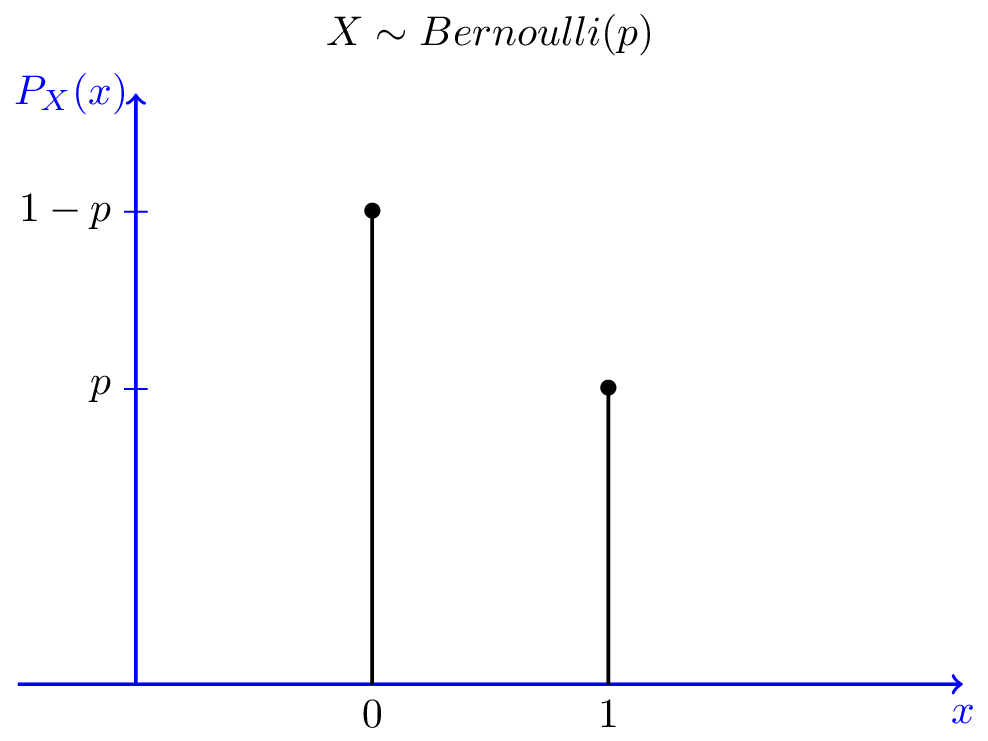
\includegraphics[width=3.75cm]{bernoulli.png}\\ \hline
		&&&\\
		{\bf Binomial} & $p_X(x)=\dbinom{n}{x}p^x(1-p)^{n-x}$, \newline\vspace*{5pt}$x=0,1,\dots,n$ & $\mathbb{E}[X]=np$ \newline\vspace*{3pt}$\var(X)=np(1-p)$ & 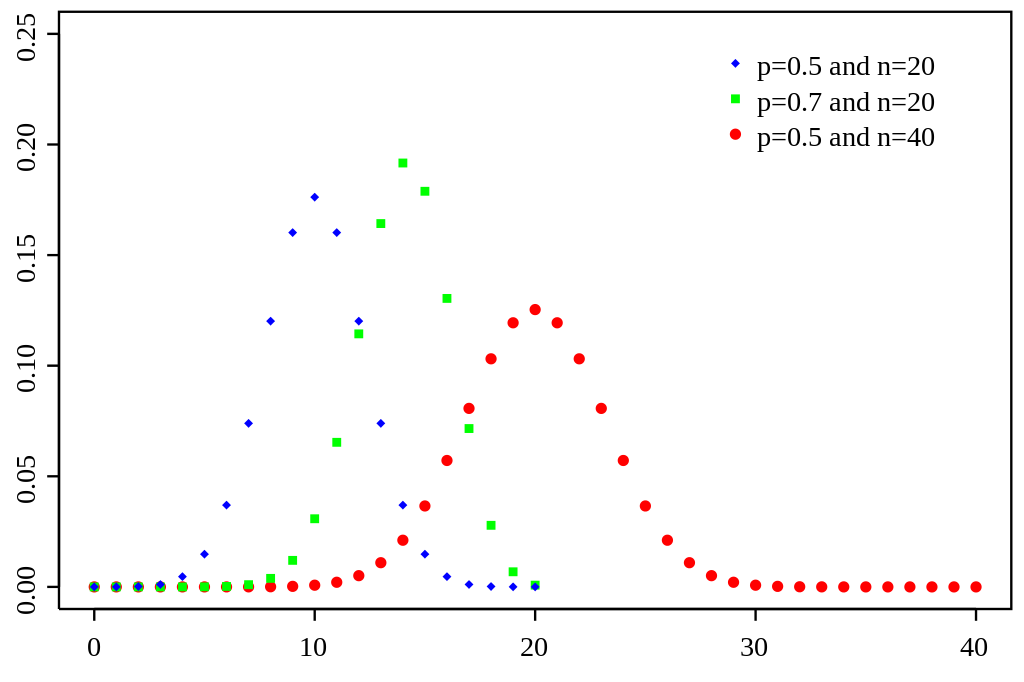
\includegraphics[width=3.75cm]{binomial.png}\\
		&&&\\ \hline
		&&&\\
		{\bf Hypergeometric} & $p_X(x)=\dfrac{\dbinom{A}{x}\dbinom{B}{n-x}}{\dbinom{A+B}{n}}$& $\mathbb{E}[X]=\dfrac{nA}{A+B}$ \newline\vspace*{3pt}$\var(X)=\dfrac{nAB}{(A+B)^2}\dfrac{A+B-n}{A+B-1}$ & 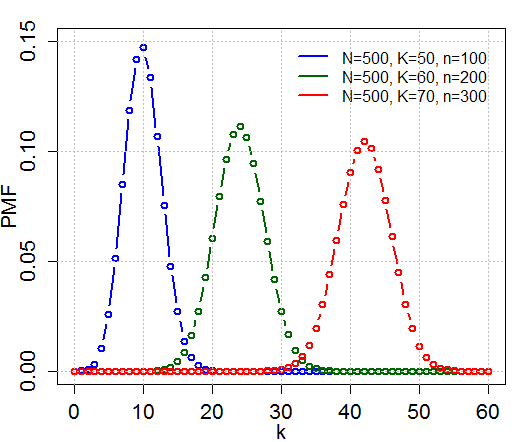
\includegraphics[width=3.75cm]{hypergeometric.png}\\
		&&&\\ \hline
		&&&\\ 
		{\bf Negative Binomial} & $p_X(k)=\dbinom{r+k-1}{k}p^k(1-p)^r$ & $\mathbb{E}[X]=\dfrac{k(1-p)}{p}$ \newline\vspace*{3pt}$\var(X)=\dfrac{r(1-p)}{p^2}$ & 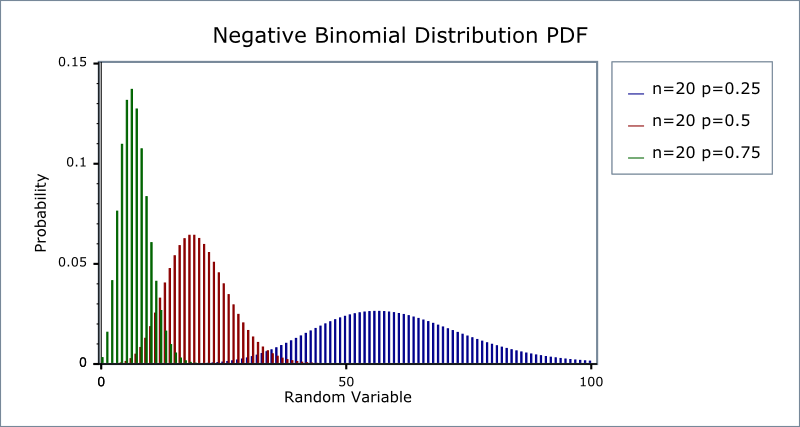
\includegraphics[width=3.75cm]{negbinomial.png}\\
		&&&\\ \hline
	\end{tabular}
\end{table}
\newpage
\begin{table}[h!]
	\begin{tabular}{| C{4.5cm} | C{7cm} | C{6cm} | C{7cm} |}
		\hline
		&&&\\
		{\bf Distribution} &
		{\bf PDF / PMF} & {\bf Expectation and Variance} & {\bf Graph} \\ 
		&&&\\ \hline
		&&&\\
		{\bf Geometric} & $p_X(k)=(1-p)^{k-1}p$ & $\mathbb{E}[X]=\dfrac{1}{p}$ \newline\vspace*{3pt}$\var(X)=\dfrac{1-p}{p^2}$ & 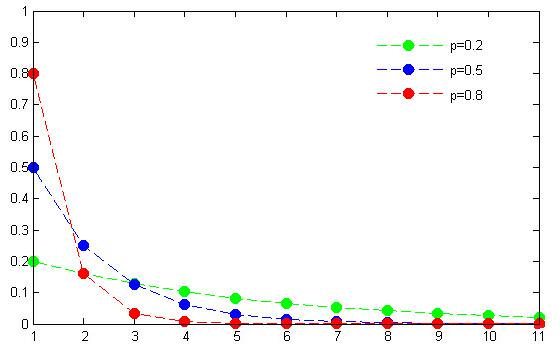
\includegraphics[width=3.75cm]{geometric.png}\\
		&&&\\ \hline
		&&&\\
		{\bf Poisson} & $p_X(k)=\dfrac{\lambda^ke^{-\lambda}}{k!}$ & $\mathbb{E}[X]=\lambda$ \newline\vspace*{3pt}$\var(X)=\lambda$ & 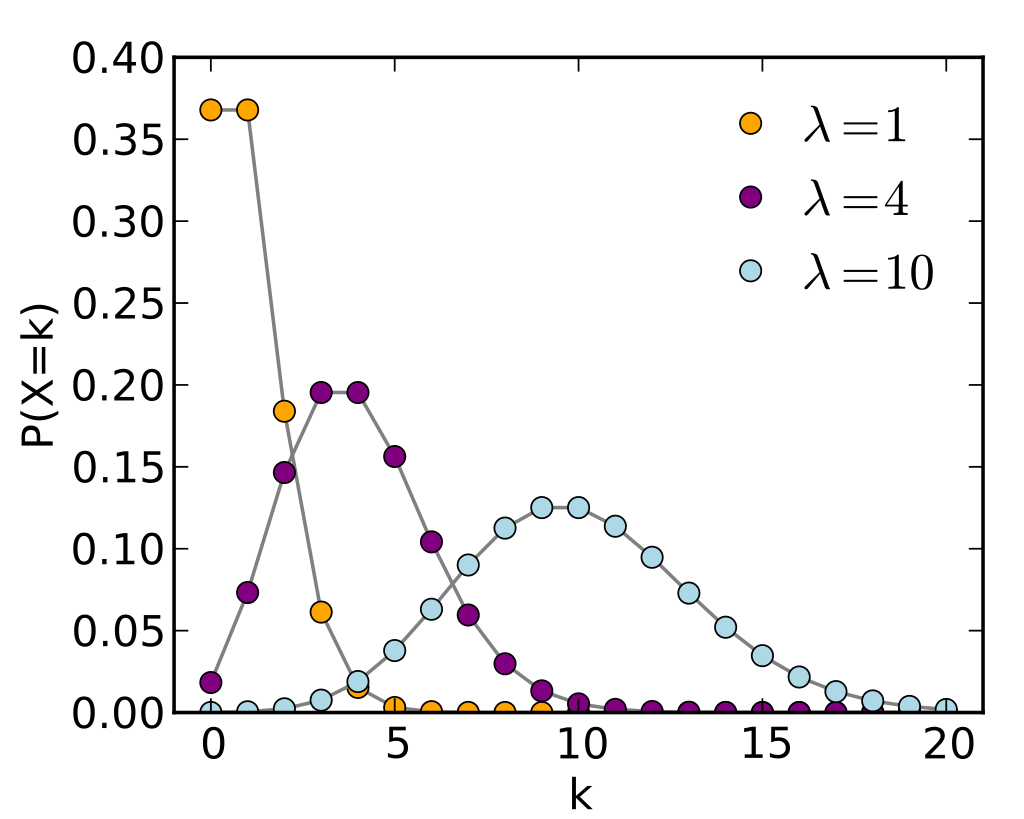
\includegraphics[width=3.75cm]{poisson.png}\\
		&&&\\ \hline
		&&&\\
		{\bf Exponential} & $f_X(x)=\lambda e^{-\lambda x}$ & $\mathbb{E}[X]=\dfrac{1}{\lambda}$ \newline\vspace*{3pt}$\var(X)=\dfrac{1}{\lambda^2}$ & 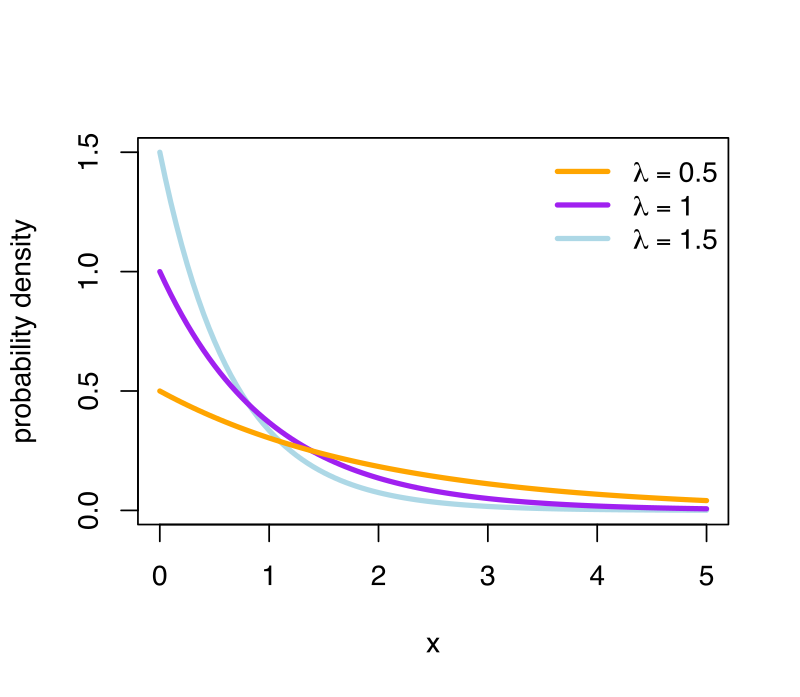
\includegraphics[width=3.75cm]{exponential.png}\\
		&&&\\ \hline
		&&&\\
		{\bf Uniform} & $f_X(x)=\dfrac{1}{b-a}$ & $\mathbb{E}[X]=\dfrac{a+b}{2}$ \newline\vspace*{3pt}$\var(X)=\dfrac{(b-a)^2}{12}$ & 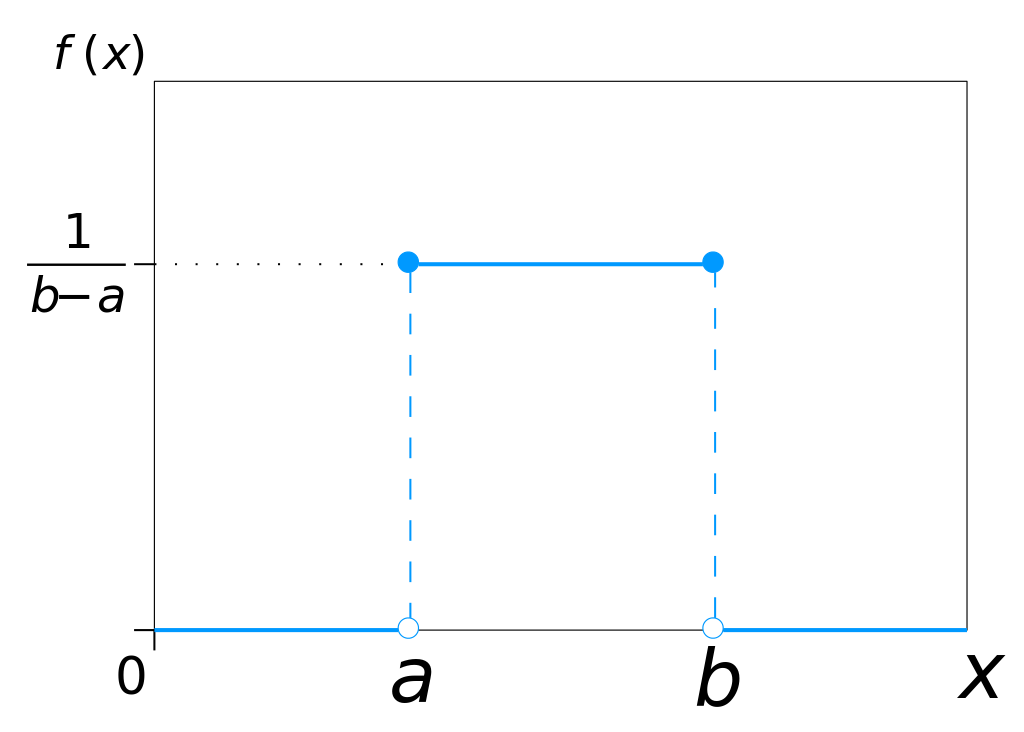
\includegraphics[width=3.75cm]{uniform.png} \\ \hline
		&&&\\
		{\bf Normal} & $f_X(x)=\dfrac{1}{\sigma\sqrt{2\pi}}e^{-\frac{(x-\mu)^2}{2\sigma^2}}$& $\mathbb{E}[X]=\mu$ \newline\vspace*{3pt}$\var(X)=\sigma^2$ & 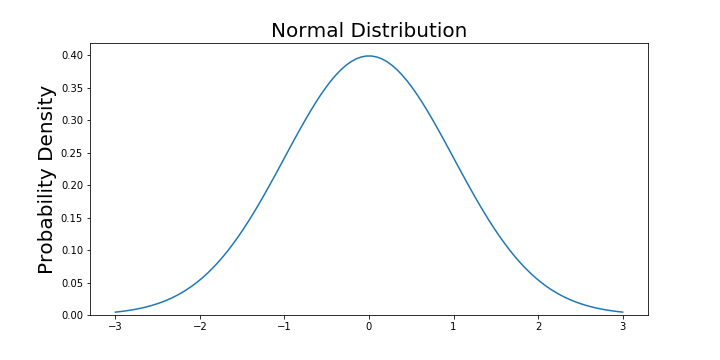
\includegraphics[width=3.75cm]{standardnormal.png}\\ \hline
	\end{tabular}
\end{table}




\end{document}
